\documentclass{amsart}%kh
%\usepackage{makeidx}
\usepackage{amssymb}
\usepackage{amsmath}
\usepackage{amsopn}
\usepackage{graphicx}
\usepackage{mathrsfs}
\usepackage{amsmath}
\usepackage{amsfonts}
\usepackage{amsthm}
\usepackage{mwe}
\usepackage{tikz}
\usepackage{pstool}
\usepackage{psfrag}
\usepackage{epstopdf}
\usepackage{pstricks}
\usepackage{tikz}
\usepackage{tikz-cd}
\usetikzlibrary{matrix,arrows,decorations.pathmorphing}
%\usepackage[T1]{fontenc}
\usepackage{textcomp}     % for \textquotesingle macro
%\usepackage{mathptmx}
 
\usetikzlibrary{matrix,arrows}
\usepackage{todonotes}
\usepackage{marginnote}
\usepackage{lettrine}
\usepackage{graphicx}
\usepackage{booktabs}
\usepackage[all]{xy}
\usepackage{enumitem}
\usepackage{latexsym}
\usepackage{eepic}
\usepackage{epsfig}
\usepackage{graphicx}
\usepackage{pst-node}
\usepackage{lipsum}
\usepackage{hyperref}
\hypersetup{
  colorlinks   = true, %Colours links instead of ugly boxes
  urlcolor     = black, %Colour for external hyperlinks
  linkcolor    = blue, %Colour of internal links
  citecolor   = red %Colour of citations
}

\usepackage{amscd}
%\usepackage{eufrak}
%\usepackage{drftcite}y
\usepackage{mathrsfs}
\usepackage[english]{babel}
%\usepackage[all,cmtip]{xy}

\usepackage[utf8]{inputenc}
\usepackage[%
    style=alphabetic,sorting=nyt,
    maxnames=10,
    sortcites=true,doi=false,
    firstinits=true,hyperref,backend=bibtex]{biblatex}
    \renewbibmacro{in:}{%
      \ifentrytype{article}{}{\printtext{\bibstring{in}\intitlepunct}}}
\usepackage[babel]{csquotes}
\usepackage{guit}
\addbibresource{References.bib}
\DeclareFieldFormat
  [article,inbook,incollection,inproceedings,patent,thesis,unpublished]
  {title}{{#1\isdot}}
\DeclareFieldFormat{pages}{#1}
%\DefineBibliographyStrings{english}{andothers={}}

\usepackage{cancel}
\AtEveryBibitem{%
\ifentrytype{book}{
    \clearfield{url}%
    \clearfield{pages}
    \clearfield{isbn}
    \clearfield{urldate}%
    \clearfield{review}%
    \clearfield{series}%%
}{}
\ifentrytype{article}{
    \clearfield{url}%
    %\clearfield{pages}
    \clearfield{issn}
    \clearfield{doi}
    \clearfield{isbn}
    \clearfield{urldate}%
    \clearfield{review}%
    %\clearfield{series}%%
}{}
\ifentrytype{collection}{
    \clearfield{url}%
    \clearfield{urldate}%
    \clearfield{review}%
    \clearfield{series}%%
}{}
\ifentrytype{incollection}{
    \clearfield{url}%
    \clearfield{urldate}%
    \clearfield{review}%
    \clearfield{series}%%
}{}
}
 \renewcommand*{\bibfont}{\small}


% better loking hyperref
% IMPORTANT: if writing math in titles, need to add "\texorpdfstring" !!
%\usepackage{hyperref}
%\hypersetup{
%   colorlinks   = true,          %Colours links instead of ugly boxes
%   urlcolor     = blue,          %Colour for external hyperlinks
%   linkcolor    = blue,          %Colour of internal links
%   citecolor   = red             %Colour of citations
%}


\numberwithin{equation}{subsection}

%
% THEOREMSTYLES, NEWTHEOREMS
%
% about theoremstyles can read here: http://en.wikibooks.org/wiki/LaTeX/Theorems


% Theorems, propositions, corollaries, lemmas
\newtheoremstyle{plain2}    % to uniformize styles with the paragraphs
   {}            % ABOVESPACE (empty value is the same as default value)
   {}            % BELOWSPACE (empty value is the same as degfault value)
   {\itshape}    % BODYFONT  (\itshape, \bfseries, \normalfont)
   {}            % INDENT (empty value is the same as 0pt, \parindent is the same as the standard indent for new paragraphs)
   {\bfseries}   % HEADFONT
   {.}           % HEADPUNCT
   {5pt plus 1pt minus 1pt}  % HEADSPACE (leave 5pt plus 1pt minus 1pt)
   {{\thmnumber{#1} \thmname{#2}{\thmnote{ (#3)}}}}          %CUSTOM-HEAD-SPEC
\theoremstyle{plain2}

\newcounter{thmc}[subsection]
\newtheorem{thm}[equation]{Theorem}
\newtheorem{theorem}[equation]{Theorem}
\newtheorem{cor}[equation]{Corollary}
\newtheorem{lemma}[equation]{Lemma}
\newtheorem{prop}[equation]{Proposition}



% Definitions, remarks, examples, claims
\newtheoremstyle{definition2}    % to uniformize styles with the paragraphs
   {}
   {}
   {\normalfont}
   {}
   {\bfseries}
   {.}
   {5pt plus 1pt minus 1pt}
   {{\thmnumber{#1} \thmname{#2}{\thmnote{#3}}}}
\theoremstyle{definition2}
\newtheorem{defi}[equation]{Definition}
\newtheorem{rem}[equation]{Remark}
\newtheorem{ex}[equation]{Example}
\newtheorem{example}[equation]{Example}
\newtheorem{cl}[equation]{Claim}
\newtheorem{cla}[equation]{Claim}



% steps (in proofs)
\newcounter{stepcounter}[subsection]
\newtheoremstyle{stepstyle}
   {}     {}
   {\normalfont}
   {\parindent}
   {\itshape}
   {}
   {5pt plus 1pt minus 1pt}
   {{\thmname{#1} \thmnumber{#2}:{\thmnote{#3}}}}
\theoremstyle{stepstyle}
\newtheorem{step}[stepcounter]{Step}



% points (look like definitions etc.)
\newtheoremstyle{point}
   {}     {}
   {\normalfont}
   {}
   {\bfseries}
   {}
   {5pt plus 1pt minus 1pt}
   {{\thmname{#1}(\thmnumber{#2})\thmnote{ #3.}}}
\theoremstyle{point}
\newtheorem{point}[equation]{}%[section]

\newcommand{\pa}[1]{\begin{point}#1\end{point}}              % shortcut
\newcommand{\Pa}[2]{\begin{point}[#1]#2\end{point}}          % To add a title. (It will look like definitions and so on)



% subpoints (look like equations)


\newtheoremstyle{subpoint}
   {}     {}            % maybe leave less space above and under?
   {\normalfont}
   {}                   % maybe add indent?
   {\normalfont}
   {}
   {5pt plus 1pt minus 1pt}
   {{\thmname{#1}{\bf (\thmnumber{#2})}\thmnote{ #3.}}}
\theoremstyle{subpoint}
\newtheorem{subpoint}[equation]{}%[section]

\newcommand{\spa}[1]{\begin{subpoint}#1\end{subpoint}}           % shortcut
\newcommand{\Spa}[2]{\begin{subpoint}[#1]#2\end{subpoint}}   % To add a title.


\newcommand{\llbracket}{[\negthinspace[}
\newcommand{\rrbracket}{]\negthinspace]}


\newcommand{\llpar}{(\negthinspace(}
\newcommand{\rrpar}{)\negthinspace)}


\newcommand{\D}{{\mathcal D}}
\newcommand{\LL}{\ensuremath{\mathbb{L}}}
\newcommand{\mL}{\ensuremath{\mathscr{L}}}
\newcommand{\mLL}{\ensuremath{\mathfrak{L}}}
\newcommand{\N}{\ensuremath{\mathbb{N}}}
\newcommand{\Z}{\ensuremath{\mathbb{Z}}}
\newcommand{\Q}{\ensuremath{\mathbb{Q}}}
\newcommand{\F}{\ensuremath{\mathbb{F}}}
\newcommand{\R}{\ensuremath{\mathbb{R}}}
\newcommand{\C}{\ensuremath{\mathbb{C}}}
\newcommand{\CP}{\ensuremath{\mathbb{CP}}}
\newcommand{\Ar}{\ensuremath{\mathscr{A}r}}
\newcommand{\Aa}{\ensuremath{\mathscr{A}}}
\newcommand{\Lm}{\ensuremath{\mathscr{L}}}
\newcommand{\OO}{\widehat{\mathscr{O}}}
\newcommand{\Pro}{\ensuremath{\mathbb{P}}}
\newcommand{\A}{\ensuremath{\mathbb{A}}}
\newcommand{\GG}{\ensuremath{\mathbb{G}}}
\newcommand{\FF}{\ensuremath{\mathbb{F}}}
\newcommand{\NN}{\ensuremath{\mathbb{N}}}
\newcommand{\G}{\ensuremath{\mathbb{G}}}
\newcommand{\X}{\ensuremath{\mathscr{X}}}
\newcommand{\scM}{\ensuremath{\mathscr{M}}}
\newcommand{\cX}{\ensuremath{\mathscr{X}}}
\newcommand{\mX}{\ensuremath{\mathfrak{X}}}
\newcommand{\mY}{\ensuremath{\mathfrak{Y}}}
\newcommand{\mK}{\ensuremath{\mathfrak{K}}}
\newcommand{\mW}{\ensuremath{\mathfrak{W}}}
\newcommand{\mH}{\ensuremath{\mathfrak{H}}}
\newcommand{\mT}{\ensuremath{\mathfrak{T}}}
\newcommand{\mm}{\ensuremath{\mathfrak{m}}}
\newcommand{\fp}{\ensuremath{\mathfrak{p}}}

\newcommand{\caM}{\ensuremath{\mathcal{M}}}
\newcommand{\caC}{\ensuremath{\mathcal{C}}}
\newcommand{\caO}{\ensuremath{\mathcal{O}}}
\newcommand{\caI}{\ensuremath{\mathcal{I}}}

\newcommand{\cA}{\ensuremath{\mathscr{A}}}
\newcommand{\cC}{\ensuremath{\mathscr{C}}}
\newcommand{\cF}{\ensuremath{\mathscr{F}}}
\newcommand{\cG}{\ensuremath{\mathscr{G}}}
\newcommand{\cH}{\ensuremath{\mathscr{H}}}
\newcommand{\cJ}{\ensuremath{\mathscr{J}}}
\newcommand{\cK}{\ensuremath{\mathscr{K}}}
\newcommand{\cL}{\ensuremath{\mathscr{L}}}
\newcommand{\cM}{\ensuremath{\mathscr{M}}}
\newcommand{\cP}{\ensuremath{\mathscr{P}}}
\newcommand{\cT}{\ensuremath{\mathscr{T}}}
\newcommand{\cU}{\ensuremath{\mathscr{U}}}
\newcommand{\cV}{\ensuremath{\mathscr{V}}}
\newcommand{\cY}{\ensuremath{\mathscr{Y}}}
\newcommand{\cZ}{\ensuremath{\mathscr{Z}}}


%\renewcommand{\exp}{\ensuremath{\mathscr{E}\mathrm{xp}}}
%\renewcommand{\log}{\ensuremath{\mathscr{L}\mathrm{og}}}
\renewcommand{\F}{\ensuremath{\mathbb{F}}}
\renewcommand{\R}{\ensuremath{\mathbb{R}}}
\renewcommand{\C}{\ensuremath{\mathbb{C}}}
\renewcommand{\Pro}{\ensuremath{\mathbb{P}}}
\renewcommand{\A}{\ensuremath{\mathbb{A}}}
\renewcommand{\X}{\ensuremath{\mathfrak{X}}}
%\renewcommand{\cX}{\ensuremath{\mathscr{X}}}
%\renewcommand{\mX}{\ensuremath{X_\infty}}
\renewcommand{\mY}{\ensuremath{\mathfrak{Y}}}
\newcommand{\mZ}{\ensuremath{\mathfrak{Z}}}
\newcommand{\mU}{\ensuremath{\mathfrak{U}}}
\newcommand{\mV}{\ensuremath{\mathfrak{V}}}
\newcommand{\mE}{\ensuremath{\mathfrak{E}}}
\newcommand{\mF}{\ensuremath{\mathfrak{F}}}
\renewcommand{\mK}{\ensuremath{K_\infty}}
\renewcommand{\cA}{\ensuremath{\mathscr{A}}}
\renewcommand{\cM}{\ensuremath{\mathscr{M}}}
\renewcommand{\cH}{\ensuremath{\mathscr{H}}}
\renewcommand{\cU}{\ensuremath{\mathscr{U}}}
\renewcommand{\cF}{\ensuremath{\mathscr{F}}}
\renewcommand{\cJ}{\ensuremath{\mathscr{J}}}
\renewcommand{\cZ}{\ensuremath{\mathscr{Z}}}
\renewcommand{\cY}{\ensuremath{\mathscr{Y}}}
\newcommand{\J}{\ensuremath{\mathscr{J}}}
\newcommand{\K}{\ensuremath{\mathscr{K}}}
\newcommand{\cR}{\ensuremath{\mathscr{R}}}

\newcommand{\Hilb}{\ensuremath{\mathrm{Hilb}}}
\newcommand{\Spec}{\ensuremath{\mathrm{Spec}\,}}
\newcommand{\Spf}{\ensuremath{\mathrm{Spf}\,}}
\newcommand{\Sp}{\ensuremath{\mathrm{Sp}\,}}
\newcommand{\Proj}{\ensuremath{\mathbb{P}}}
\newcommand{\Ima}{\mathrm{Im}}
\newcommand{\Lie}{\mathrm{Lie}}
\newcommand{\Pic}{\mathrm{Pic}}
\newcommand{\ord}{\mathrm{ord}}
\newcommand{\redu}{\mathrm{red}}
\newcommand{\pr}{\mathrm{pr}}
\newcommand{\mult}{\mathrm{mult}}
%\newcommand{\gcd}{\mathrm{gcd}}
\newcommand{\nor}{\mathrm{nor}}
\newcommand{\prin}{\mathrm{prin}}
\newcommand{\lcm}{\mathrm{lcm}}
\newcommand{\Jac}{\mathrm{Jac}}
\newcommand{\im}{\mathrm{im}}
\newcommand{\tame}{\mathrm{tame}}
\newcommand{\Var}{\mathrm{Var}}
\newcommand{\Gal}{\mathrm{Gal}}
\newcommand{\Hom}{\mathrm{Hom}}
\newcommand{\coker}{\mathrm{coker}}
\newcommand{\an}{\mathrm{an}}
\newcommand{\sm}{\mathrm{sm}}
\newcommand{\et}{\mathrm{\acute{e}t}}
\newcommand{\Gr}{\mathrm{Gr}}
\newcommand{\Art}{\mathrm{Art}}
\newcommand{\Sw}{\mathrm{Sw}}
\newcommand{\pot}{\mathrm{pot}}
\newcommand{\length}{\mathrm{length}}

\newcommand{\divisor}{\mathrm{div}}
\newcommand{\weight}{\mathrm{wt}}
\newcommand{\lift}{\mathrm{lift}}
\newcommand{\spl}{\mathrm{spl}}
\newcommand{\free}{\mathrm{free}}
\newcommand{\tors}{\mathrm{tors}}
\newcommand{\ab}{\mathrm{ab}}
\newcommand{\tor}{\mathrm{tor}}
%\newcommand{\Hom}{\mathrm{Hom}}
\newcommand{\sh}{\mathrm{sh}}
%\newcommand{\sm}{\mathrm{sm}}
\newcommand{\qc}{\mathrm{qc}}
\newcommand{\ur}{\mathrm{ur}}
\newcommand{\rank}{\mathrm{rank}}
%\newcommand{\Gal}{\mathrm{Gal}}
\newcommand{\tr}{\mathrm{tr}}
\newcommand{\Trace}{\mathrm{Trace}}
\newcommand{\ess}{\mathrm{ess}}
\newcommand{\lct}{\mathrm{lct}}
\newcommand{\Sk}{\mathrm{Sk}}
\newcommand{\gp}{\mathrm{gp}}

\def\trank#1{t(#1)}
\def\ttame#1{t_{\tame}(#1)}
\def\tpot#1{t_{\pot}(#1)}
\def\comp#1{\phi(#1)}
\def\Comp#1{\Phi(#1)}
\def \degree{\colon\!}
\def\dgr#1#2{\mbox{$[#1\degree #2]$}}
\def\CompS#1{S^{\Phi}_{#1}}



\hyphenpenalty=6000 \tolerance=10000


\title{TITLE}
\author{Morgan Brown and Enrica Mazzon}
\date{}


\begin{document}
\maketitle

%\begin{abstract}
%Given a variety $X$ over a complete discretely valued field, we define the skeleta associated to log-regular models of $X$. Their construction relies on the notion of the Kato fan, determines simplicial subsets of the Berkovich space $X^\an$ and generalises the Berkovich skeleta introduced by Musta\c{t}\u{a} and Nicaise.
%
%Combining the logarithmic framework with the properties of the weight function, we study the skeleta of products and symmetric quotients of varieties. As an application, we show that, if $X$ is a $\text{K}3$ surface admitting a log-regular model with reduced special fibre, then the essential skeleton of $\Hilb^n(X)$ coincides with the $n$-symmetric product of the essential skeleton of $X$.
%\end{abstract}


\section{Introduction}
%
%\subsection{Berkovich skeleta.} Let $R$ be a complete discrete valuation ring, with residue field $k$ and quotient field $K$. Let $X$ be a smooth and proper $K$-variety. In \cite{Berkovich1990}, Berkovich developed a theory of analytic geometry over $K$. He associated a $K$-analytic space to $X$; each point corresponds to a real valuation on the residue field of a point of $X$, extending the discrete valuation on $K$. This space, denoted by $X^\an$, is called the Berkovich space associated to $X$.
%
%In order to construct points in the Berkovich space, we consider the geometry of models of $X$. An \textit{snc} model $\cX$ of $X$ is a regular flat separated scheme of finite type over $R$, such that the generic fibre $\cX_K$ is isomorphic to $X$ and the special fibre $\cX_k$ is a strict normal crossing divisor. By strict normal crossing, we mean that its irreducible components are regular and intersect transversally, but the divisor is not necessarily reduced. From any snc model $\cX$ of $X$ one can construct a subspace of $X^\an$, called the Berkovich skeleton of $\cX$ and denoted by $\Sk(\cX)$: it is homeomorphic to the dual intersection complex of the divisor $\cX_k$ \cite{MustataNicaise}.
%
%The Berkovich skeleta turn out to be relevant in the study of the topology of $X^\an$. Firstly, they shape the Berkovich space, as $X^\an$ is homeomorphic to the inverse limit $\underleftarrow{\lim}\Sk(\cX)$ where $\cX$ runs through all snc models of $X$. Secondly, the homotopy type of $X^\an$ is determined by any snc model $\cX$: indeed, Berkovich and Thuiller proved that $\Sk(\cX)$ is a strong deformation retract of $X^\an$.
%
%\subsection{The skeleton of a log-regular model.} In this paper we define a logarithmic version of the Berkovich skeleton by considering log-regular models of $X$. More precisely, let $\cX$ be an integral flat separated scheme of finite type over $R$ such that the logarithmic scheme $\cX^+$, endowed with the divisorial structure induced by the special fibre, is a log-regular log scheme. Roughly speaking, this amounts to imposing a weaker condition on the special fibre $\cX_k$ than being strict normal crossing: it expresses that the pair $(\cX,\cX_k)$ has a toroidal structure.
%
%To any such log scheme $\cX^+$, in \cite{Kato1994a} Kato attached a combinatorial structure $F_\cX$ called a \emph{fan}: it consists of the set of the generic points of intersections of irreducible components of $\cX_k$ equipped with a sheaf of monoids. In particular, the theory of Kato fans provides a suitable framework to encode toroidal modifications of $\cX$ in terms of subdivisions of the Kato fan $F_\cX$.
%
%Any log-regular model $\cX^+$ of $X$ gives rise to a polyhedral complex in $X^\an$, whose faces correspond to the points of the Kato fan $F_\cX$: it is again called the skeleton $\Sk(\cX^+)$. As one would expect, this construction coincides with the previous definition of skeleton in the case of an snc model. Many of the properties that hold true for skeleta of snc models continue to hold in the more general case of log-regular models.
%
%The significance of having this generalisation is that some of the tools to study the Berkovich skeleta can be conveniently interpreted in logarithmic terms. For example, in \cite{MustataNicaise} Musta\c{t}\u{a} and Nicaise defined the \textit{weight function} $\weight_{\omega}$ on $X^\an$ associated to a pluricanonical form $\omega$ on $X$; its value at points of the skeleton of an snc model of $X$ can be computed by means of an explicit and more manageable formula using logarithmic differential forms. Moreover, in the following we prove that the formula expressed in the logarithmic language can be also generalised to the skeleton of a log-regular model (Proposition \ref{prop weight function log formula}).
%
%\subsection{The essential skeleton.}It is natural to ask if, among all the Berkovich skeleta, we can construct a \textit{canonical} skeleton that is uniquely determined and that, at the same time, captures as much information as possible about the geometry of $X^\an$. In \cite{MustataNicaise}, Musta\c{t}\u{a} and Nicaise gave a positive answer to the question by defining the \textit{essential skeleton} $\Sk(X)$ of $X$: it is a finite simplicial complex in $X^\an$, depends only on the variety $X$ and constitutes a new birational invariant of $X$.
%
%The definition of the essential skeleton is based on the weight functions $\weight_{\omega}$ on $X^\an$. Indeed, given any snc model $\cX$ of $X$, the points of $\Sk(\cX)$ where $\weight_{\omega}$ reaches its minimal value single out certain faces of $\Sk(\cX)$ that only depend on $X$ and $\omega$. The essential skeleton $\Sk(X)$ is defined as the union of these minimizing loci over all the non-zero pluricanonical forms $\omega$ of $X$.
%
%One may wonder if the essential skeleton may be realised as the skeleton of a distinguished model of $X$. It was proved in \cite{NicaiseXu} that, when the canonical line bundle of $X$ is semi-ample, the essential skeleton can be identified with the dual intersection complex of the special fibre of any minimal \textit{dlt} model of $X$. This means that, up to enlarging the class of models and admitting mild singularities, the essential skeleton is still the skeleton of a model of $X$. The main advantage of this second approach relies on the possibility of applying results from the birational geometry of minimal dlt models. In particular, taking advantage of the techniques of the Minimal Model Program and following \cite{deFernexKollarXu2012}, one can conclude that the essential skeleton is a strong deformation retract of $X^\an$ \cite{NicaiseXu}.
%
%While the importance of the essential skeleton in the pursuit of a canonical and geometrically significant skeleton was emphasised already in previous works, at least two interesting aspects have yet to be explored. Firstly, whether it is feasible to find alternative proofs of existing results or to determine further properties of the essential skeleton, adopting the ``weight function approach'' and only relying on the geometric structure of $X^\an$ instead of the geometry of minimal dlt models. Secondly, it would be interesting to explore more the relation between the variety $X$ and the essential skeleton $\Sk(X)$, to identify the information about $X$ that is encoded in $\Sk(X)$.
%
%In the present work, we will prove results in both of these directions when X is a Hilbert scheme of points on a $\text{K}3$ surface.
%
%\subsection{The essential skeleton of the Hilbert scheme of $n$ points on a $\text{K3}$ surface.} Our main theorem asserts that the essential skeleton of the Hilbert scheme of $n$ points on a $\text{K}3$ surface $S$ is homeomorphic to the $n$-th symmetric product of the essential skeleton of $S$, i.e. $\Sk(\Hilb^n(S)) \simeq \text{Sym}^n(\Sk(S))$, assuming that $S$ admits a log-regular model with reduced special fibre and that $k$ is algebraically closed (Theorem \ref{thm essential skeleton hilb}).
%
%It has been observed that many natural operations in algebraic geometry commute with passing to the skeleton (or tropicalization). Typical examples include the results that the skeleton of a moduli space of curves is the moduli space of the corresponding tropical curves \cite{AbramovichCaporasoPayne} and the skeleton of the Jacobian of a curve is the tropical Jacobian of the skeleton of the curve \cite{BakerRabinoff}. Our main theorem can be interpreted as a new instance of this phenomenon (since skeleta have no infinitesimal structure, their ``Hilbert schemes of points'' are simply given by their symmetric powers). 
%
%The main inspiration for Theorem \ref{thm essential skeleton hilb} is an ongoing project by Gulbrandsen, Halle, Hulek and Zhang, following \cite{GulbrandsenHalleHulek} and \cite{GulbrandsenHalleHulek2016}. Their investigation focuses on the degenerations of Hilbert schemes of points and provides, as an application, an analogue result about the essential skeleton of Hilbert schemes, but only in the particular case of type II degeneration of $K3$ surfaces. The techniques involved differ a lot. Indeed, their approach is based on the method of \textit{expanded degenerations}, which first appeared in \cite{Li}, and on the construction of suitable GIT quotients. Furthermore, to perform this construction on a variety, they need a combinatorial assumption on the special fibre of a model of the variety.
%
%In particular, in the case of a $\text{K}3$ surface $S$ over $K$, the GIT quotient they form turns out to be a minimial dlt model of the Hilbert scheme of $n$ points on $S$. We recall that, by \cite{NicaiseXu}, the essential skeleton of a variety can be identified with the dual complex of any minimal dlt model of the variety. Hence, it follows that the GIT quotient they construct provides a description of the essential skeleton of $\Hilb^n(X)$. Finally, in accord with our result, they also conclude that the dual complex in question is the $n$-th symmetric product of the essential skeleton of $S$.
%%One can extend the notion of essential skeleta to singular varieties as follows: it is defined as the essential skeleton of any resolution of singularities. This is well-defined by the birational invariance of the essential skeleton. Combining this with the fact that $\Hilb^n(X)$ is a desingularisation of the $n$-th symmetric product $\text{Sym}^n(X)$ (\cite{Fogarty}), we see that the essential skeleton of $\Hilb^n(X)$ can be identified with the essential skeleton of $\text{Sym}^n(X)$. Therefore, our claim is that $\Sk(\text{Sym}^n(X))$ is homeomorphic to $\text{Sym}^n(\Sk(X))$. This means that the operation of quotienting the product structure by the action of the symmetric group $\mathfrak{S}_n$ is compatible with passing to the essential skeleton. This provides evidence that, in the case of a $\text{K}3$ surface and its Hilbert scheme, the essential skeleta are related in the same way as the varieties themselves are related.
%
%\subsection{A sketch of the proof.} Let us now briefly indicate the main ideas of the proof. The arguments only rely on the properties of the weight function and the notion of skeleta for log-regular models. In particular, minimal dlt models do not play a role in our proof. 
%
%By the birational invariance of the essential skeleton, we are reduced to studying the essential skeleton of $\text{Sym}^n(S)$. Hence, we want to study its behaviour when we consider products and symmetric quotients.
%
%The first part of the proof consists in showing that the essential skeleton of the product may be identified with the product of the essential skeleta, i.e. $\Sk(X^n) \simeq (\Sk(X))^n$ (Corollary \ref{cor semistability and essential skeleta}). This result holds for every Calabi-Yau variety X over $K$ with a log-regular model with reduced special fibre.
%
%We start by studying the relation between the skeleton of a product of two such varieties $X$ and $Y$ with the product of the corresponding skeleta. The logarithmic setting turns out to be the most suitable. Firstly, the product of log-regular models $\cX^+$ and $\cY^+$ of $X$ and $Y$ is a log-regular model $\cZ^+$ of $Z=X\times_K Y$. So we can consider the skeleta of all three of these log-regular models and compare them. Secondly, let $\omega_{X}$ and $\omega_Y$ be canonical forms on $X$ and $Y$. Thanks to the weight function formula in terms of logarithmic differentials, we are able to relate the points in $\Sk(\cZ^+)$ that minimise the weight function $\weight_{\pr_X^*\omega_K \otimes \pr_Y^*\omega_Y}$ to pairs of points in $\Sk(\cX^+)$ and $\Sk(\cY^+)$ that minimise respectively $\weight_{\omega_X}$ and $\weight_{\omega_Y}$ (Paragraph \ref{paragraph weight function product}). The technical requirements of the algebraic closedness of $k$ and the existence of a log-regular model with reduced special fibre guarantee a good understanding of the product in the category of log schemes (Proposition \ref{prop semistability and skeleta}).
%
%The second part of the proof focuses on the $n$-th symmetric product of $X$: we conclude that the essential skeleton of the $n$-th symmetric product of $X$ may be identified with the quotient of the product of $n$ copies of the essential skeleton, i.e. $\Sk(X^n/\mathfrak{S}_n) \simeq (\Sk(X))^n / \mathfrak{S}_n$ (Corollary \ref{cor semistability and essential skeleta quotient}). Let $\omega$ be a canonical form on $X^n$ invariant under $\mathfrak{S}_n$, so that it induces a canonical form on the quotient $X^n/\mathfrak{S}_n$. The main technical results involved in this second part state that not only the minimal values attained by $\weight_{\omega}$ on $(X^n)^\an$ and $(X^n/\mathfrak{S}_n)^\an$ coincide (see (\ref{equ equality weight})), but also that the set of points on $(X^n/\mathfrak{S}_n)^\an$ of minimal weight is equal to the image via $(X^n)^\an \rightarrow (X^n/\mathfrak{S}_n)^\an$ of the points of minimal weight on $(X^n)^\an$ (Proposition \ref{prop KS of quotient}). This leads to the expected explicit description of the essential skeleton of the quotient $S^n/\mathfrak{S}_n$, hence of $\Hilb^n(S)$ by birational invariance of the essential skeleton.

%\subsection{Structure of the paper.} To conclude this introduction, we give a brief overview of the structure of the paper. In Section \ref{sect fs product} we recall the definition of fine and saturated products in the category of log schemes. In Section \ref{sect kato fan} we explain the construction of the Kato fan associated  to a log-regular log scheme, as proposed in \cite{Kato1994a}, and we provide a description of the Kato fan of a product of log-regular log schemes. In Section \ref{sect skeleton log} we introduce the technical core of the paper, the notion of the skeleton associated to a log-regular model. We show that it is a simplicial subset of the Berkovich space and generalises the Berkovich skeleta in \cite{MustataNicaise}.
%
%The applications of this construction are discussed in the second half of the paper. In Section \ref{sect wt log} we study the properties of the weight function in connection with the skeleta of log-regular models. In Section \ref{sect an of symm product} we focus on the symmetric product of a variety, proving that its essential skeleton is related to the essential skeleton of the standard product. Our main result is discussed in Section \ref{sect essential sk Hilb}, where we give a precise characterization of the essential skeleton of the Hilbert scheme of points on a $\text{K}3$ surface. 
%
%\subsection{Acknowledgements.}

\subsection{Notation.}
\spa{Let $R$ be a complete discrete valuation ring with maximal ideal $\mm$, residue field $k=R/\mm$ and quotient field $K$. We assume that the valuation $v_K$ is normalized, namely $v_K(\pi)=1$ for any uniformizer $\pi$ of $R$. We define by $|\cdot|_K= \exp(- v_K(\cdot))$ the absolute value on $K$ corresponding to $v_K$; this turns $K$ into a non-archimedean complete valued field.}
\spa{ We write $S=\Spec R$ and we denote by $s$ the closed point of $S$. Let $\cX$ be an $R$-scheme of finite type. We will denote by $\cX_k$ the special fiber of $\cX$ and by $\cX_K$ the generic fibre. Moreover, we will denote by $\widehat{\cX}$ the $\mm$-adic completion of $\cX$ and by $\widehat{\cX}_\eta$ the generic fiber of $\widehat{\cX}$ in the category of $K$-analytic spaces.}

\spa{Let $X$ be a proper $K$-scheme. A model for $X$ over $R$ is a flat separated $R$-scheme $\cX$ of finite type endowed with an isomorphism of $K$-schemes $\cX_K \rightarrow X$. If $X$ is smooth over $K$,
we say that $\cX$ is an snc model for $X$ if it is regular over $R$, and the
special fiber $\cX_k$ is a strict normal crossings divisor on $\cX$. In equicharacteristic $0$, such a model always exists, by Hironaka's resolution of singularities.}

\spa{ \label{sss-log} All log schemes in this paper are  fine and saturated (\emph{fs}) log schemes and defined with respect to the Zariski topology. We denote a log scheme by $\cX^+=(\cX,\caM_{\cX})$, where $\caM_{\cX}$ is the structural sheaf of monoids. We denote by $$\mathcal{C}_{\cX}=\mathcal{M}_{\cX}/\mathcal{O}_{\cX}^{\times}$$
the characteristic sheaf of $\cX^+$. The sheaf $\mathcal{C}_{\cX}$
is a Zariski sheaf on $\cX^+$, supported on $\cX_k$; if $\cX^+$ is log-regular, then $\caC_{\cX}$ is a constructible sheaf.
For every point $x$ of $\cX_k$, we denote by $\mathcal{I}_{\cX,x}$
the ideal in $\mathcal{O}_{\cX,x}$ generated by
$$\mathcal{M}_{\cX,x}\setminus \mathcal{O}_{\cX,x}^{\times}.$$ We denote
by $S^+$ the scheme $S$ endowed with the standard log structure
(the divisorial log structure induced by $s$). If an $R$-scheme $\cX$ is given, we will always denote by $\cX^+$ the log scheme over $S^+$ that we obtain by endowing $\cX$ with the divisorial log structure associated with
$\cX_k$.

If $\cX^+$ is a log-regular log scheme over $S^+$, then the locus where the log structure is non-trivial is a divisor that we will denote by $D_{\cX}$. Thus, the log structure on $\cX^+$ is the divisorial log structure induced by $D_{\cX}$, by \cite{Kato1994a}, Theorem 11.6.

}

\spa{Let $(X,\Delta_X)$ be a pair where $X$ is a proper $K$-scheme, $\Delta_X$ is an effective $\Q$-divisor such that $\Delta_X= \sum a_i \Delta_{X,i}$ with $0 \leqslant a_i \leqslant 1$, and $X^+=(X,\lceil \Delta_X \rceil)$ is a log-regular log scheme over $K$. A log-regular log scheme $\cX^+$ over $S^+$ is a model for $(X,\lceil \Delta_X \rceil)$ over $S^+$ if $\cX$ is a model of $X$ over $R$, the closure of any component of $\Delta_X$ in $\cX$ has non-empty intersection with $\cX_k$, and $D_\cX = \overline{\lceil \Delta_X \rceil} + \cX_{k,\redu}$. }

\spa{We say that a log-regular log scheme $\cX^+$ over $S^+$ is semistable if the divisor $D_\cX$ is reduced. We say that a proper $K$-variety X has semistable reduction if it admits an $R$-model $\cX$ such that $\cX^+$ is log-smooth over $S^+$, with reduced special fiber; such a model is called a semistable model of $X$. This is a weaker notion than requiring the existence of an snc-model with reduced special fibre.}

\spa{We denote by $(\cdot)^{\an}$ the analytification functor from the category of $K$-schemes of finite type to Berkovich's category of $K$-analytic spaces. For every $K$-scheme of finite type $X$, as a set, $X^{\an}$ consists of the pairs $x=(\xi_x,|\cdot|_x)$ where $\xi_x$ is a point of $X$ and $|\cdot|_x$ is an absolute value on the residue field $\kappa(\xi_x)$ of $X$ at $\xi_x$ extending the absolute value $|\cdot|_K$ on $K$. We endow $X^{\an}$ with the Berkovich topology, i.e. the weakest one such that \begin{itemize}
\item[(i)] the forgetful map $\phi: X^{\an} \rightarrow X$, defined as $(\xi_x,|\cdot|_x) \mapsto \xi_x$, is continuous,
\item[(ii)] for any Zariski open subset $U$ of $X$ and any regular function $f$ on $U$ the map $|f|:\phi^{-1}(U) \rightarrow \R$ defined by $|f|(\xi_x,|\cdot|_x)=|f(\xi_x)|$ is continuous. 
\end{itemize}}

\section{The Kato fan of a log-regular log scheme} \label{sect kato fan}

\subsection{Definition of Kato fans.}
\spa{ According to \cite{Kato1994a}, Definition 9.1, a monoidal space $(T, \caM_T)$ is a topological space $T$ endowed with a sharp sheaf of monoids $\caM_T$, where \textit{sharp} means that $\caM_{T,t}^\times = \{1\}$ for every $t \in T$. We often simply denote the monoidal space by $T$.

A morphism of monoidal spaces is a pair $(f,\varphi):(T,\caM_T) \rightarrow (T',\caM_{T'})$  such that $f:T \rightarrow T'$ is a continuous function of topological spaces and $\varphi: f^{-1}(\caM_T) \rightarrow \caM_{T'}$ is a sheaf homomorphism such that $\varphi_{t}^{-1}(\{1\})=\{1\}$ for every $t \in T$.}

\begin{example}
If $\cX^+$ is a log scheme then the Zariski topological space $\cX$ is equipped with a sheaf of sharp monoids $\caC_{\cX}$, the characteristic sheaf of $\cX^+$. Thus $(\cX,\caC_{\cX})$ is a monoidal space. Moreover, morphisms of log schemes
induce morphisms of characteristic sheaves, hence morphism of monoidal spaces. We therefore obtain a functor from the category of log schemes to the category of monoidal spaces.
\end{example}

\begin{example}
Given a monoid $P$, we may associate to it a monoidal space called the spectrum of $P$. As a set, $\Spec P$ is the set of all prime ideals of $P$. The topology is characterized by the basis open sets $D(f)= \{ \fp \in \Spec P | f \notin \fp \}$ for any $f \in P$. The monoidal sheaf is defined by $$\caM_{\Spec P} (D(f))= S^{-1}P / (S^{-1}P)^{\times}$$ where $S=\{f^n | n \geqslant 0\}$.
\end{example}

\spa{A monoidal space isomorphic to the monoidal space $\Spec P$ for some monoid $P$ is called an affine Kato fan. A monoidal space is called a Kato fan if it has an open covering consisting of affine Kato fans. In particular, we call a Kato fan integral, saturated, of finite type or $fs$ if it admits a cover by the spectra of monoids with the respective properties.}

\spa{A morphism of fs Kato fans $F' \rightarrow F$ is called a \emph{subdivision} if it has finite fibres and the morphism $$\Hom(\Spec \N, F') \rightarrow \Hom (\Spec \N, F)$$ is a bijection. Allowing subdivisions a Kato fan might take the following shape.
\begin{prop} \label{kato subdivision}(\cite{Kato1994a}, Proposition 9.8)
Let $F$ be a $fs$ Kato fan. Then there is a subdivision $F' \rightarrow F$ such that $F'$ has an open cover $\{U'_i\}$ by Kato cones with $U'_i \simeq \Spec \N^{r_i}$. 
\end{prop}
The strategy of the proof of Proposition \ref{kato subdivision} goes back to \cite{KempfKnudsenMumfordEtAl1973} and relies on a sequence of particular subdivisions of the Kato fan, the so-called star and barycentric subdivisions (\cite{AbramovichChenMarcusEtAl2015}, Example 4.10).}

\subsection{Kato fans associated to log-regular log schemes.}
\begin{thm}\label{kato fan associated} (\cite{Kato1994a}, Proposition 10.2)
Let $\cX^+$ be a log-regular log scheme. Then there is an initial strict morphism $(\cX, \caC_{\cX}) \rightarrow F$ to a Kato fan in the category of monoidal spaces. Explicitly, there exist a Kato fan $F$ and a morphism $\pi: (\cX, \caC_{\cX}) \rightarrow F$ such that $\pi^{-1}(\caM_{F}) \simeq \caC_{\cX}$ and any other morphism to a Kato fan factors through $\pi$.
\end{thm}
The Kato fan $F$ in Theorem \ref{kato fan associated} is called the Kato fan associated to $\cX^+$; it is the topological subspace of
$\cX$ consisting of the points $x$ such that the maximal ideal $\mathfrak{m}_x$ of
$\mathcal{O}_{\cX,x}$ is equal to $\mathcal{I}_{\cX,x}$, and
$\mathcal{M}_F$ is the inverse image of $\mathcal{C}_{\cX}$ on
$F$, henceforth we write $\caC_F$ for $\caM_F$.

\begin{example} \label{example kato fan regular model}
Assume that $\cX$ is regular, of finite type over $S$ and $\cX_k$ is a divisor with strict
normal crossings. Then $\cX^+$ is log-regular and $F$ is the set
of generic points of intersections of irreducible components of
$\cX_k$. For each point $x$ of $F$, the stalk of $\mathcal{C}_F$
is isomorphic to $(\N^r,+)$, with $r$ the number of irreducible
components of $\cX_k$ that pass through $x$.
\end{example}

This example admits the following partial generalisation.

\begin{lemma} \label{lemma points Kato fan}
Let $\cX^+$ be a log-regular log scheme. Then the fan $F$ consists of the generic points of intersections of irreducible components of $D_{\cX}$.
\end{lemma}
\begin{proof}
First, we show that every such generic point is a point of $F$. Let $E_1,\ldots,E_r$ be irreducible components of $D_{\cX}$ and let $x$ be a generic point of the intersection $E_1\cap\ldots\cap E_r$. We set $d=\dim \mathcal{O}_{\cX,x}$. Since $\cX^+$ is log-regular, we know that $\mathcal{O}_{\cX,x}/\mathcal{I}_{\cX,x}$ is regular and that \begin{equation} \label{equ log regularity}
d=\dim \mathcal{O}_{\cX,x}/\mathcal{I}_{\cX,x}+\mathrm{rank}\,\mathcal{C}^{\gp}_{\cX,x}.\end{equation} We denote by $V(\caI_{\cX,x})$ the vanishing locus of the ideal $\caI_{\cX,x}$ in $\cX$.
We want to prove that $\caI_{\cX,x}= \mathfrak{m}_x$. We assume the contrary, hence that $\caI_{\cX,x} \subsetneq \mathfrak{m}_x$. This assumption implies that there exists $j$ such that $V(\caI_{\cX,x}) \nsubseteq E_j$: indeed, if the vanishing locus is contained in each irreducible component $E_i$, i.e. $$V(\caI_{\cX,x}) \subseteq E_1 \cap \ldots \cap E_r \subseteq \overline{\{x\}},$$ then $\caI_{\cX,x} \supseteq \mathfrak{m}_x$. From the assumption of log-regularity it follows that the vanishing locus $V(\caI_{\cX,x})$ is a regular subscheme, and moreover that $\cX^+$ is Cohen-Macaulay by \cite{Kato1994a}, Theorem 4.1. Thus, there exists a regular sequence $(f_1,\ldots,f_l)$ in $\caI_{\cX,x}$ where $l$ is the codimension of $V(\caI_{\cX,x})$, i.e. $$ \dim \mathcal{O}_{\cX,x}/\mathcal{I}_{\cX,x} = d-l.$$ Moreover by the equality (\ref{equ log regularity}), $\mathrm{rank}\,\mathcal{C}^{\gp}_{\cX,x} = l$.
 
We claim that the residue classes of these elements $f_i$ in $\mathcal{C}_{\cX,x}^{\gp}$ are linearly independent. Assume the contrary. Then, up to renumbering the $f_i$, there exist an  integer $e$ with $1< e< l$, non-negative integers $a_1,\ldots,a_l$, not all zero, and a unit $u$ in $\mathcal{O}_{\cX,x}$ such that $$f_1^{a_1}\cdot \ldots \cdot f_{e-1}^{a_{e-1}}=u\cdot f_e^{a_e}\cdot \ldots \cdot f_l^{a_l}.$$ This contradicts the fact that $(f_1,\ldots,f_l)$ is a regular sequence in $\mathcal{I}_{\cX,x}$. Thus, the classes $\overline{f_1}, \ldots,\overline{f_l}$ are independent in $\caC_{\cX,x}^\gp$. As we also have the equality $\mathrm{rank}\,\mathcal{C}^{\gp}_{\cX,x}=l$, it follows that these classes generate $\caC_{\cX,x}^\gp \otimes_{\Z} \Q$.

Let $g_j$ be a non-zero element of the ideal $\caI_{\cX,x}$ that vanishes along $E_j$: it necessarily exists as otherwise $E_j$ is not a component of the divisor $D_{\cX}$. Then $g_j$ satisfies $$g_{j}^N = v \cdot f_1^{b_1} \cdot \ldots \cdot f_l^{b_l}$$ with $b_i \in \Z$, $v$ a unit in $\caO_{\cX,x}$ and $N$ a positive integer. As $g_j$ vanishes along the irreducible component $E_j$, at least one of the functions $f_1,\ldots,f_l$ has to vanish along $E_j$: assume that is $f_1$.

On the one hand, as $f_1$ is identically zero on $E_j$, the trace of $E_j$ on $V(\caI_{\cX,x})$ has at most codimension $l-1$ in $E_j$ at the point $x$. On the other hand, we assumed that $V(\caI_{\cX,x})$ is not contained in $E_j$ and it has codimension $l$ in $\caO_{\cX,x}$. Then, the trace of $E_j$ on $V(\caI_{\cX,x})$ has codimension $l$ in $E_j$ at $x$. This is a contradiction. We conclude that the ideal $\caI_{\cX,x}$ is equal to the maximal ideal $\mathfrak{m}_x$, therefore $x$ is a point of $F$.

It remains to prove the converse implication: every point $x$ of the fan $F$ must be a generic point of an intersection of irreducible components of $D_{\cX}$. Let $x$ be a point of $F$: by construction of Kato fan $F$, the maximal ideal of $\mathcal{O}_{\cX,x}$ is equal to $\mathcal{I}_{\cX,x}$, thus it is generated by elements in $\mathcal{M}_{\cX,x}$. The zero locus of such an element is contained in $D_{\cX}$ by definition of the logarithmic structure on $\cX^+$. Therefore, the zero locus is a union of irreducible components of the trace of $D_{\cX}$ on $\Spec \mathcal{O}_{\cX,x}$ and $x$ is a generic point of the intersection of all such irreducible components.
\end{proof}

\begin{rem}
By convention, the generic point of the empty intersection of irreducible components is the generic point of $\cX$. By definition, this point is also included in the Kato fan $F$. Thus, for example, the Kato fan associated to $S^+$ consists of two points: the generic point of $S$ that corresponds to the empty intersection, and the closed point $s$ corresponding to the unique irreducible component of the logarithmic divisorial structure.  
\end{rem}

Moreover, the example \ref{example kato fan regular model} also leads to the following characterization.

\begin{prop} \label{resolution log scheme kato fan} (\cite{GabberRamero}, Corollary 12.5.35)
Let $\cX^+$ be a log-regular log scheme over $S^+$ and $F$ its associated Kato fan. The following are equivalent: \begin{enumerate}
\item for every $x \in F$, $M_{F,x} \simeq \N^{r(x)}$,
\item the underlying scheme $\cX$ is regular.
\end{enumerate}
If this is the case, then the special fibre $\cX_k$ is a strict normal crossing divisor.
\end{prop}
\spa{The construction of the Kato fan of a log scheme defines a functor from the category of log-regular log schemes to the category of Kato fans. Indeed, given a morphism of log schemes $\cX^+ \rightarrow \cY^+$, we consider the embedding of the associated Kato fan $F_{\cX}$ in $\cX^+$ and the canonical morphism $\cY^+ \rightarrow F_{\cY}$: the composition $$F_{\cX} \hookrightarrow \cX^+ \rightarrow \cY^+ \rightarrow F_\cY$$ functorially induces a map between associated Kato fans. Moreover, this association preserves strict morphisms (\cite{Ulirsch2013}, Lemma 4.9).}
\subsection{Resolutions of log schemes via Kato fan subdivisions.} \label{section resolution via kato subd}
\begin{prop} (\cite{Kato1994a}, Proposition 9.9) \label{prop morphism induced by subdivision kato fan}
Let $\cX^+$ be a log-regular log scheme and let $F$ be its associated Kato fan. Let $F' \rightarrow F$ be a subdivision of fans. Then there exist a log scheme ${\cX'}^+$, a morphism of log schemes ${\cX'}^+ \rightarrow \cX^+$ and a commutative diagram
\begin{center}
$\begin{gathered}
\xymatrixcolsep{2pc} \xymatrix{
  (\cX', \caC_{\cX'}) \ar[r]^-{p} \ar[d]^{} & F' \ar[d]^{}\\
  (\cX, \caC_{\cX}) \ar[r]^-{\pi_{\cX}}   & F
}
\end{gathered}$\end{center}such that $p^{-1}(\caM_{F'}) \simeq \caC_{\cX'}$, they define a final object in the category of such diagrams and the refinement $F'\to F$ is induced by the morphism of log-regular log schemes $\cX'^+ \rightarrow \cX^+$.
\end{prop}

\spa{\label{rem resolution via subd}
It follows that given any subdivision $F' \rightarrow F$ of the Kato fan F associated with a log regular log scheme $\cX^+$, we can construct a log scheme over $\cX^+$ with prescribed associated Kato fan $F'$. Combining this fact with Proposition \ref{kato subdivision} and Proposition \ref{resolution log scheme kato fan} yields to the construction of resolutions of log schemes in the following sense: for any log-regular log scheme over $S^+$ we can find a birational modification by a regular log scheme with strict normal special fibre. Moreover, the morphism of log schemes ${\cX'}^+ \rightarrow \cX^+$ is obtained by a log blow-up  (\cite{Niziol2006}, Theorem 5.8).} 


\subsection {Fibred products and associated Kato fans.}\label{sect fs product}
\spa{Given morphisms of \emph{fs} log schemes $f_1: \cX_1^+ \rightarrow \cY^+$ and $f_2: \cX_2^+ \rightarrow \cY^+$, their fibred product exists in the category of log schemes. It is obtained by endowing the usual fibred product of schemes
\begin{equation} \label{fibered product diagram}
\begin{gathered}
\xymatrixcolsep{3pc} \xymatrix{
  \cX_1\times_{\cY} \cX_2 \ar[r]^-{p_1} \ar[dr]^-{p_{\cY}} \ar[d]^-{p_2} & \cX_1 \ar[d]^{f_1}\\
  \cX_2 \ar[r]^{f_2}   & \cY
}
\end{gathered}
\end{equation}
with the log structure associated to $p_1^{-1}\caM_{\cX_1} \oplus_{p_{\cY}^{-1}\caM_{\cY}} p_2^{-1}\caM_{\cX_2}$. If $u_1:P \rightarrow Q_1$ and $u_2:P \rightarrow Q_2$ are charts for the morphisms $f_1$ and $f_2$ respectively, then the induced morphism $\cX_1\times_{\cY} \cX_2 \rightarrow \Spec \Z[Q_1 \oplus_P Q_2]$ is a chart for $\cX_1^+\times_{\cY^+} \cX_2^+$. }

\spa{In general, the fibred product is not $fs$, but the category of $fs$ log schemes also admits fibred products. Keeping the same notations, the following is a chart of the fibred product in the category of fine and saturated log schemes $$\cX_1^+\times_{\cY^+}^{\text{fs}} \cX_2^+ = (\cX_1^+\times_{\cY^+} \cX_2^+) \times_{\Z[Q_1 \oplus_P Q_2]} \Z[(Q_1 \oplus_P Q_2)^{\text{sat}}]$$(\cite{Bultot2015}, 3.6.16). We remark that the two fibre products above may not only have different log structures, but also the underlying schemes may differ. Nevertheless, this does not occur when the monoid $Q_1 \oplus_P Q_2$ is saturated.}

\spa{Log smoothness is preserved under fs base change and composition (\cite{GabberRamero}, Proposition 12.3.24). In particular, if $f_1: \cX_1^+ \rightarrow \cY^+$ is log-smooth and $\cX_2^+$ is log-regular, then $\cX_1^+\times^{\text{fs}}_{\cY^+} \cX_2^+$ is log-regular, by \cite{Kato1994a}, Theorem 8.2.

Consider log-smooth morphisms of fs log schemes $\cX_1^+ \rightarrow \cY^+$ and $\cX_2^+ \rightarrow \cY^+$. The sheaves of logarithmic differentials are related by the following isomorphism \begin{equation} \label{equ kahler diff product}
p_1^* \Omega^{\log}_{\cX_1^+/\cY^+} \oplus p_2^* \Omega^{\log}_{\cX_2^+/ \cY^+} \simeq \Omega^{\log}_{\cX_1^+\times^{\text{fs}}_{\cY^+} \cX_2^+ /\cY^+}\end{equation} by \cite{GabberRamero}, Proposition 12.3.13. Furthermore, by assumption of log-smoothness over $S^+$ the logarithmic differential sheaves are locally free of finite rank (\cite{Kato1994a}, Proposition 3.10) and we can consider their determinants; they are called log canonical bundles and denoted by $\omega^{\log}$. The following isomorphism is a direct consequence of (\ref{equ kahler diff product}) \begin{equation} \label{equ log can bundles}
p_1^* \omega^{\log}_{\cX_1^+/\cY^+} \otimes p_2^* \omega^{\log}_{\cX_2^+/ \cY^+} \simeq \omega^{\log}_{\cX_1^+\times^{\text{fs}}_{\cY^+} \cX_2^+ /\cY^+}.\end{equation} }

\spa{Similarly to the construction of fibred products of $fs$ log schemes, the category of $fs$ Kato fans admits fibred products: on affine Kato fans $F=\Spec P$ and $G=\Spec Q$ over $H=\Spec T$, $F\times_{H}G$ is the spectrum of the amalgamated sum $(P \oplus_T Q)^{\text{sat}}$ in the category of $fs$ monoids (\cite{Ulirsch2016}, Proposition 2.4) and on the underlying topological spaces, this coincides with the usual fibred product.}
We seek to compare the Kato fan associated to the fibred product of log-regular log schemes with the fibred product of associated Kato fans.
\begin{prop} \label{local isomo kato fan product}(\cite{Saito2004}, Lemma 2.8) Given $\mathscr{T}^+$ a log-regular log scheme, let $\cX^+$ and $\cY^+$ be log-smooth log schemes over $\mathscr{T}^+$. We denote by $\cZ^+$ the $fs$ fibred product $\cX^+\times^{\text{fs}}_{\mathscr{T}^+} \cY^+$. Then, the natural morphisms $F_{\cZ}\to F_{\cX}$ and $F_{\cZ}\to F_{\cY}$ induce a morphism of Kato fans \begin{equation} \label{equ local isomo kato fans}
F_{\cZ} \rightarrow F_{\cX} \times_{F_{\mathscr{T}}} F_{\cY}
\end{equation} that is locally an isomorphism.
\end{prop}

\spa{For any pair of points $(x,y)$ in $F_\cX \times_{F_{\mathscr{T}}} F_\cY$, we denote by $n(x,y)$ be the number of preimages of $(x,y)$ in the Kato fan of $\cZ^+$ under the local isomorphism (\ref{equ local isomo kato fans}).
\begin{lemma} \label{lemma number of preimages} If $x'$ is in the closure of $x$, and $y'$ in the closure of $y$, then $n(x',y')\geqslant n(x,y)$.
\end{lemma}
\begin{proof}
Let $z'$ be a preimage of the pair $(x',y')$. By Proposition \ref{local isomo kato fan product}, there exists an open neighbourhood $U_{z'}$ of $z'$ such that the restriction of $F_{\cZ} \rightarrow F_{\cX} \times_{F_\mathscr{T}} F_{\cY}$ to $U_{z'}$ is an isomorphism onto its image. In particular, $(x,y)$ lies in this image. Thus, there exists a unique preimage of $(x,y)$ that is contained in $U_{z'}$. It follows that $n(x',y')\geqslant n(x,y)$.
\end{proof}
}

\subsection{Semistability and Kato fans associated to the fibred products.} 
\spa{\textcolor{red}{change style} We investigate a sufficient condition, for pairs of points whose closures intersect the special fibre, to turn the local isomorphism (\ref{equ local isomo kato fans}) into an isomorphism: it concerns the notion of semistability. We recall that a log-regular log scheme $\cX^+$ is said to be semistable if the divisor $D_{\cX}$, where the log structure is non-trivial, is reduced.}

\spa{In order to see the relevance of the assumption of semistability, we need some results on saturated morphism of log schemes. We recall that, locally around a point $x$ of the divisor $D_{\cX}$, the morphism of characteristic monoids $\N \rightarrow \caC_{\cX,x}$ is a saturated morphism of monoids if, for any morphism $u: \N \rightarrow P$ of $fs$ monoids, the amalgamated sum $\caC_{\cX,x} \oplus_{\N} P$ is still saturated.

Following the work by T. Tsuji in an unpublished 1997 preprint, Vidal in \cite{Vidal} defines the saturation index of a morphism of \emph{fs} monoids. In the case of log-regular log scheme over $S^+$ it can be easily computed: it is the least common multiple of the multiplicities of the prime components of the divisor $D_{\cX}$. The following criterion holds.
\begin{lemma} \label{lemma criterion saturation}(\cite{Vidal}, Section 1.3)
A morphism of fs monoids is saturated if and only if the saturation index is equal to 1.
\end{lemma}
}

\begin{prop} \label{prop semistability and iso Kato fans}
Assume that the residue field $k$ is algebraically closed. Let $\cX^+$ and $\cY^+$ be log-smooth log scheme over $S^+$. Let $\cZ^+$ be their $fs$ fibred product. If $\cX^+$ is semistable, then for any pair of points $(x,y)$ in $F_\cX \times_{F_S} F_\cY$ whose closures intersect the special fibres $\cX_k$ and $\cY_k$ respectively, the morphism $F_{\cZ}\xrightarrow{} F_{\cX} \times F_{\cY},$ induced by the projections $\cZ^+ \rightarrow \cX^+$ and $\cZ^+ \rightarrow \cY^+$, is a bijection above the pair $(x,y)$, namely $n(x,y)=1$.
\end{prop}

\begin{proof}
By hypothesis $\cX^+$ is a semistable log-regular log scheme over $S^+$, hence the saturation index of $\cX^+ \rightarrow S^+$ is 1. Thus, by Lemma \ref{lemma criterion saturation} the morphism of log schemes $\cX^+ \rightarrow S^+$ induces a saturated morphism of characteristic monoids at every point of $\cX^+$. The saturation condition implies that the fibred product in the category of log schemes coincides with the fibred product in the category of $fs$ log schemes. In particular, the underlying scheme of $\cZ^+$ coincides with the usual schematic fibred product, hence its points are characterized as follows:$$z=(x,y,s,\fp) \text{ and } \caO_{\cZ,z}=(\caO_{\cX,x} \otimes_R \caO_{\cY,y})_{\fp}$$ where $x$ and $y$ are points of $\cX^+$ and $\cY^+$ both mapped to the same point $s$ of $S$, while $\fp$ is a prime ideal of the tensor product of residue fields $\kappa(x) \otimes_{\kappa(s)} \kappa(y)$. We look for a characterization of points $z$ in $\cZ^+$ that lie in the Kato fan $F_{\cZ}$.

If the point $z$ lies in $F_{\cZ}$, then the maximal ideal $\mathfrak{m}_z$ is equal to the ideal $\caI_{\cZ,z}$ by definition. By the flatness of the models $\cX^+$ and $\cY^+$ over $S^+$, the morphisms of local rings $\caO_{\cX,x} \rightarrow \caO_{\cZ,z}$ and $\caO_{\cY,y} \rightarrow \caO_{\cZ,z}$ are injective. Hence, the equalities $\mathfrak{m}_x= \caI_{\cX,x}$ and $\mathfrak{m}_y= \caI_{\cY,y}$ hold. Thus, the points $z$ in $\cZ^+$ that lie in the Kato fan $F_{\cZ}$ are necessarily points such that the projections $x$ and $y$ to $\cX^+$ and $\cY^+$ lie in their associated Kato fans. Therefore, we may assume $x \in F_{\cX}$, $y \in F_{\cY}$, and it remains to characterize the prime ideals $\fp$ such that $z=(x,y,s,\fp) \in F_{\cZ}$.

By log-regularity of $\cZ^+$, the point $z$ lies in the associated Kato fan if and only if $\dim \caO_{\cZ,z}= \rank \caC_{\cZ,z}^{\text{gp}}$. At the level of characteristic sheaves it holds that $$\rank \caC_{\cZ,z}^{\text{gp}}= \rank \caC_{\cX,x}^{\text{gp}} + \rank \caC_{\cY,y}^{\text{gp}} - 1.$$ Since $x$ and $y$ are both assumed to be points in the associated Kato fans, the equality between dimension of local rings and rank of the groupifications of characteristic sheaves lead to the equivalence \begin{align*}
z \in F_{\cZ}  \Leftrightarrow \dim \caO_{\cZ,z} & = \rank \caC_{\cZ,z}^{\text{gp}} = \rank \caC_{\cX,x}^{\text{gp}} + \rank \caC_{\cY,y}^{\text{gp}} - 1 \\
& = \dim \caO_{\cX,x} +  \dim \caO_{\cY,y} -1.
\end{align*}
By log-regularity of $\cZ^+$, it holds that $\dim \caO_{\cZ,z} \geqslant \rank \caC_{\cZ,z}^{\text{gp}}$, thus the inequality $$\dim \caO_{\cZ,z} \geqslant \dim \caO_{\cX,x} +  \dim \caO_{\cY,y} -1$$ is always true and equality holds only for minimal prime ideals $\fp$ of $\kappa(x) \otimes_{\kappa(s)} \kappa(y)$. Therefore, in order to determine the number $n(x,y)$ of preimages of $(x,y)$ in $F_\cZ$, we need to study the number of minimal prime ideals of the tensor product $\kappa(x) \otimes_{\kappa(s)} \kappa(y)$. 

If $s$ is the closed point of $S$, then its residue field is the algebraically closed field $k$. It follows that the tensor product $\kappa(x) \otimes_{k} \kappa(y)$ is a domanin, hence it has a unique minimal prime ideal, namely $0$. We obtain that $n(x,y)=1$ for any pair of points of $F_\cX \times_{F_S} F_\cY$ that lie in the special fibres.

Let $(x,y)$ be a pair of points in $F_\cX \times_{F_S} F_\cY$ whose closures intersect the special fibres, namely there exist $x' \in F_\cX \cap \cX_k$ and $y' \in F_\cY \cap \cY_k$ such that $x'$ is in the closure of $x$ and $y'$ in the closure of $y$. Then, by the previous part of the proof and by Lemma \ref{lemma number of preimages}, we have $n(x,y) \leqslant n(x',y') =1$. 
%Otherwise, we denote by $\mathscr{V}$ the closure of $x$ in $\cX^+$: it is still a log-smooth scheme over $S^+$ with reduced special fibre $\mathscr{V}_k$. We denote by $L$ the separable closure of $\kappa(s)$ in $\kappa(x)$ and by $O_L$ its valuation ring. Let $\mathscr{V}_{O_L}$ be the base change of $\mathscr{V}$ to $\Spec(O_L)$: the generic fibre $\mathscr{V}_L$ is normal, as normality is preserved under separable field extension,
%%lemma 32.10.6 Stack project % 
%and the special fibre is still reduced. By \cite{Liu2002}, Lemma 4.1.18, it follows that $\mathscr{V}_{O_L}$ is normal. Since $\mathscr{V}_{O_L}$ is normal and proper with reduced special fibre, $\mathscr{V}_L$ is connected.
%%lemma 36.26.7 Stack project %
%We deduce that $\kappa(s)$ is separably algebraically closed in $\kappa(x)$. Finally by \cite{DieudonneGrothendieck}, Proposition 4.3.2, the tensor product $\kappa(x) \otimes_{\kappa(s)} \kappa(y)$ has a unique minimal prime ideal.
\end{proof}

\section{The skeleton of a log-regular log scheme} \label{sect skeleton log}
\subsection{Construction of the skeleton of a log-regular log scheme.}

\spa{Let $\cX^+$ be a log-regular log scheme over $S^+$. Let $x$ be a point of the associated Kato fan $F$. Denote by $F(x)$ the set of points
$y$ of $F$ such that $x$ lies in the closure of $\{y\}$, and by
$\mathcal{C}_{F(x)}$ the restriction of $\mathcal{C}_F$ to $F(x)$.
Denote
 by $\Spec \mathcal{C}_{\cX,x}$ the spectrum of the monoid
$\mathcal{C}_{\cX,x}=\mathcal{C}_{F,x}$. Then there exists a
canonical isomorphism of
 monoid spaces
$$(F(x),\mathcal{C}_{F(x)})\to \Spec \mathcal{C}_{\cX,x}:y\mapsto \{s\in \mathcal{C}_{\cX,x}\,|\,s(y)= 0\}$$ where the expression $s(y)= 0$ means that $s'(y)= 0$ for any representative $s'$ of $s$ in $\mathcal{M}_{\cX,x}$. In particular, we obtain a bijective correspondence between the faces of the monoid $\mathcal{C}_{\cX,x}$ and the points of $F(x)$, and for every point $y$ of $F(x)$, a surjective cospecialization morphism of monoids $$\tau_{x,y}:\mathcal{C}_{\cX,x}\to \mathcal{C}_{\cX,y}$$ which induces an isomorphism of monoids $$S^{-1}\mathcal{C}_{\cX,x}/(S^{-1}\mathcal{C}_{\cX,x})^{\times}\cong \mathcal{C}_{\cX,x}/S \xrightarrow{\sim}
 \mathcal{C}_{\cX,y}$$ where $S$ denotes the monoid of elements $s$ in $\mathcal{C}_{\cX,x}$ such that $s(y)\neq 0$.}

\spa{For each point $x$ in $F$, we denote by $\sigma_x$ the set of morphisms of monoids $$\alpha:\mathcal{C}_{\cX,x}\to (\R_{\geq 0},+)$$ such that $\alpha(\pi)=1$ for every uniformizer $\pi$ in $R$. We endow $\sigma_x$ with the topology of pointwise covergence, where $\R_{\geq 0}$ carries the usual Euclidean topology. Note that $\sigma_x$ is a polygon, possibly semiopen, in the real affine space
$$\{\alpha:\mathcal{C}^{\gp}_{\cX,x}\to (\R,+)\,|\,\alpha(\pi)=1\mbox{ for every uniformizer }\pi\mbox{ in
}R\}.$$ If $y$ is a point of $F(x)$, then the surjective
cospecialization morphism $\tau_{x,y}$ induces a topological
embedding $\sigma_y\to \sigma_x$ that identifies $\sigma_y$ with a face of $\sigma_x$.}

\spa{We denote by $T$ the disjoint union of the topological
spaces $\sigma_x$ with $x$ in $F$. On the topological space $T$, we consider the equivalence relation $\sim$ generated by couples of the form $(\alpha,\alpha\circ \tau_{x,y})$ where $x$ and $y$ are points in $F$ such that $x$ lies in the closure of $\{y\}$ and $\alpha$ is a point of $\sigma_y$.

The skeleton of $\cX^+$ is defined as the quotient of the topological space $T$ by the equivalence relation $\sim$. We denote this skeleton by $\Sk(\cX^+)$. It is clear that $\Sk(\cX^+)$ has the structure of a polyhedral complex with cells $\{\sigma_x,\,x\in F\}$ and that the faces of a cell $\sigma_x$ are precisely the cells $\sigma_y$ with $y$ in $F(x)$. 
}

\spa{ \label{rem points in kato fan and skeleton}
We note that $\sigma_x$ is empty for any point $x$ that does not lie in the special fibre $\cX_k$: indeed, outside the special fibre any uniformizer is an invertible element, so it is trivial in $\caC_{\cX,x}$ and is mapped to $0$ by any morphism of monoids. Therefore, the construction of the skeleton associated to $\cX^+$ only concerns the points in the Kato fans $F$ that lie in the special fibre. In particular, given a generic point $x \in \cX_k$ of an intersection of components of $D_\cX$, where at least one component is not in the special fibre, the corresponding face $\sigma_x$ is unbounded.

In other words, the skeleton associated to a log-regular scheme $\cX^+$, where $D_\cX$ allows horizontal components, generalizes Berkovich's skeleta by admitting unbounded faces in the direction of the horizontal components. It also generalizes the construction performed by Gubler, Rabinoff and Werner in \cite{GublerRabinoffWerner} of a skeleton associated to a strictly semistable pair.
}
 
\subsection{Embedding the skeleton in the non-archimedean generic fiber.}
\spa{Let $\cX^+$ be a log-regular log scheme over $S^+$. Let $x$ be a point of the associated Kato fan $F$. As the log structure on $\cX^+$ is of finite type, the characteristic monoid $\caC_{\cX,x}$ is of finite type too, and thus $\caC_{\cX,x}^\gp$ is a free abelian group of finite rank. Hence there exists a section $$\zeta: \caM_{\cX,x}^\gp / \caM_{\cX,x}^\times \rightarrow \caM_{\cX,x}^\gp.$$ The section $\zeta$ restricts to $\caC_{\cX,x} \rightarrow \caM_{\cX,x}$; indeed, if $x \in \caM_{\cX,x}$ then $\zeta(\overline{x})-x \in \caM_{\cX,x}^\times$. Therefore we may choose a section \begin{equation}\label{eq:sect}\mathcal{C}_{\cX,x}\to
\mathcal{M}_{\cX,x}\end{equation} of the projection homomorphism
$$\mathcal{M}_{\cX,x}\to \mathcal{C}_{\cX,x}$$ and use this section to view $\mathcal{C}_{\cX,x}$ as a submonoid of $\mathcal{M}_{\cX,x}$. Note that $\mathcal{C}_{\cX,x}\setminus \{0\}$ generates the ideal $\caI_{\cX,x}$ of $\mathcal{O}_{\cX,x}$.
\\

We propose a generalisation of \cite{MustataNicaise}, Lemma 2.4.4. \begin{lemma} \label{lemma admissible expansion} Let $A$ be a Noetherian ring, let $I$ be an ideal of $A$ and let $(y_1,\ldots,y_m)$ be a system of generators for $I$. We denote by $\hat{A}$ the $I$-adic completion of $A$. Let $B$ be a subring of $A$ such that the elements $y_1,\ldots,y_m$ belong to $B$ and generate the ideal $B \cap I$ in $B$. Then, in the ring $\hat{A}$, every element $f$ of $B$ can be written as \begin{equation} \label{equ lemma admiss form}
f=\sum_{\beta \in \Z^m_{\geqslant 0}} c_\beta y^\beta
\end{equation} where the coefficients $c_\beta$ belong to $((A\setminus I) \cap B) \cup \{0\}$.
\end{lemma} 
\begin{proof}
Let $f$ be an element of $B$, we construct an expansion for $f$ of the form (\ref{equ lemma admiss form}) by induction. If $f$ belongs to the complement of $I$, the conclusion trivially holds. Otherwise, $f$ belongs to $I$ and we can write $f$ as a linear combination of the elements $y_1,\ldots,y_m$ with coefficients in $B$: $$f= \sum_{j=1}^{m} b_j y_j, \quad b_j \in B.$$

By induction hypothesis, we suppose that $i$ is a positive integer and that we can write every $f$ in $B$ as a sum of an element $f_i$ of the form (\ref{equ lemma admiss form}) and a linear combination of degree $i$ monomials in the elements $y_1,\ldots, y_m$ with coefficients in $B$. We apply this assumption to the coefficients $b_j$, hence
$$b_j=b_{j,i} + \sum_{\substack{\beta \in \Z^m_{\geqslant 0} \\|\beta|=i}} b_{j,\beta} y^\beta, \quad b_{j, \beta} \in B.$$ Then we can write $f$ as a sum of an element $f_{i+1}$ of the form (\ref{equ lemma admiss form}) and a linear combination of degree $i+1$ monomials in the elements $y_1,\ldots,y_m$ with coefficients in $B$
$$ f=\underbrace{\sum_{j=1}^{m} b_{j,i} y_j}_{f_{i+1}} + \sum_{j=1}^{m}\Big( \sum_{\substack{\beta \in \Z^m_{\geqslant 0} \\|\beta|=i}} b_{j,\beta} y^\beta \Big) y_j$$ such that $f_i$ and $f_{i+1}$ have the same coefficients in degree less or equal to $i$. Iterating this construction we finally find an expansion of $f$ of the required form.
\end{proof}}

\spa{ \label{paragr admissible expansion}Let $f$ be an element of $\mathcal{O}_{\cX,x}$. Considering $A=B=\caO_{\cX,x}$, $I=\mathfrak{m}_x$ and a system of generators for $\mathfrak{m}_x$ in $\caC_{\cX,x} \setminus \{1\}$, by Lemma \ref{lemma admissible expansion} we can write $f$ as a formal power series
\begin{equation}\label{eq-adm}
f=\sum_{\gamma \in \mathcal{C}_{\cX,x}}c_{\gamma}\gamma
\end{equation}
 in
$\widehat{\mathcal{O}}_{\cX,x}$, where each coefficient $c_\gamma$
 is either zero or a unit in $\mathcal{O}_{\cX,x}$. We call this formal series an \textit{admissible expansion} of $f$. We set
 \begin{equation}\label{equ def S}
S=\{\gamma\in\mathcal{C}_{\cX,x}\,|\,c_\gamma\neq 0\}
 \end{equation} and we denote by $\Gamma_x(f)$ the set of elements of $S$ that lie on a compact face of the convex hull of $S+ \mathcal{C}_{\cX,x}$ in $\mathcal{C}^{\gp}_{\cX,x}\otimes_{\Z}\R$. We call $\Gamma_x(f)$ the {\em initial support} of $f$ at $x$ and we remark that the notation  makes sense in view of the next proposition.}
\begin{prop}\label{prop-init}\item
\begin{enumerate}
\item \label{it:indep1} The element
$$f_x=\sum_{\gamma\in \Gamma}c_\gamma(x) \gamma\quad \in k(x)[\mathcal{C}_{\cX,x}]$$ depends on the choice of the section \eqref{eq:sect}, but not on the expansion \eqref{eq-adm}. \item \label{it:indep2} The subset $\Gamma$ of $\mathcal{C}_{\cX,x}$ only depends on $f$ and $x$, and not on the choice of the section \eqref{eq:sect} or the expansion \eqref{eq-adm}.
\end{enumerate}
\end{prop}
\begin{proof}
If we denote by $I$ the ideal of $k(x)[\mathcal{C}_{\cX,x}]$ generated by $\mathcal{C}_{\cX,x}\setminus \{1\}$, then it follows from \cite{Kato1994a} that there exists an isomorphism of $k(x)$-algebras \begin{equation} \label{equ isomo graded algebras}
\mathrm{gr}_I \,k(x)[\mathcal{C}_{\cX,x}]\to \mathrm{gr}_{\mathfrak{m}_x}\, \mathcal{O}_{\cX,x}.
\end{equation}
Using this result and following the argument of  \cite{MustataNicaise} Proposition 2.4.6, we show that $f_x$ does not depend on the expansion of $f$. Let $$f=\sum_{\gamma \in \mathcal{C}_{\cX,x}}c'_{\gamma}\gamma$$ be another admissible expansion of $f$ with associated set $\Gamma'$ and element $f'_x$. Then $$0=\sum_{\gamma \in \mathcal{C}_{\cX,x}}(c_{\gamma}- c'_\gamma)\gamma =\sum_{\gamma \in \mathcal{C}_{\cX,x}}d_{\gamma}\gamma$$ where the right hand side is an admissible expansion obtained by choosing admissible expansions for the elements $c_\gamma-c'_\gamma$ that do not lie in $\caO_{\cX,x}^\times \cup \{0\}$. In particular $d_\gamma(x)= c_\gamma(x)-c'_\gamma(x)$ for any $\gamma$ in $ \Gamma_x \cup \Gamma'_x$. The isomorphism of graded algebras in (\ref{equ isomo graded algebras}) implies that the elements $d_\gamma$ must all vanish, hence $\Gamma_x = \Gamma'_x$ and $f_x=f'_x$.  

Point \eqref{it:indep2} follows from the fact that the coefficients $c_\gamma$ of $f_x$ are independent of the chosen section up to multiplication by a unit in $\mathcal{O}_{\cX,x}$, so that the support $\Gamma$ of $f_x$ only depends on $f$ and $x$.
\end{proof}



\begin{prop}\label{prop-val}
Let $x$ be a point of $F$ and let $$\alpha:\mathcal{C}_{\cX,x}\to (\R_{\geq 0},+)$$ be an element of $\sigma_x$.Then there exists a unique minimal real valuation $$v:\mathcal{O}_{\cX,x} \setminus \{0\}\to \R_{\geq 0}$$ such that $v(m)=\alpha(\overline{m})$ for each element $m$ of $\mathcal{M}_{\cX,x}$.
\end{prop}
\begin{proof}
We will prove that the map
\begin{equation}\label{eq:val}
v:\mathcal{O}_{\cX,x} \setminus \{0\}\to \R:f\mapsto
\min\{\alpha(\gamma)\,|\,\gamma\in \Gamma_x(f)\}\end{equation}
satisfies the requirements in the statement. We fix a section $$\mathcal{C}_{\cX,x}\to \mathcal{M}_{\cX,x}.$$
It is straightforward to check that $(f\cdot g)_x=f_x\cdot g_x$ for all $f$ and $g$ in $\mathcal{O}_{\cX,x}$. This implies that $v$ is a valuation. It is obvious that
$v(m)=\alpha(\overline{m})$ for all $m$ in $\mathcal{M}_{\cX,x}$, since we can write $m$ as the product of an element of $\mathcal{C}_{\cX,x}$ and a unit in $\mathcal{O}_{\cX,x}$.

Now we prove minimality.Consider any real valuation $$w:\mathcal{O}_{\cX,x}\to \R$$ such that $w(f)=\alpha(\overline{m})$ for each element $m$ of
$\mathcal{M}_{\cX,x}$, and let $f$ be an element of
$\mathcal{O}_{\cX,x}$. We must show that $w(f)\geq v(f)$.

We set $$C_{\alpha}=\mathcal{C}_{\cX,x}\setminus \alpha^{-1}(0).$$ We denote by $I$ the ideal in $\mathcal{O}_{\cX,x}$ generated by $C_{\alpha}$ and by $A$ the $I$-adic completion of $\mathcal{O}_{\cX,x}$. By Lemma \ref{lemma admissible expansion}, we see that we can write $f$ in $A$ as \begin{equation} \label{equ expasion wrt I}
\sum_{\beta \in C_{\alpha}\cup\{1\}}d_\beta \beta
\end{equation} where $d_\beta$ is either zero or contained in the complement of $I$ in $\mathcal{O}_{\cX,x}$.

Since $\alpha(\beta)>0$ for every $\beta\in C_{\alpha}$, we can find an integer $N>0$ such that $w(g)>w(f)$ for every element $g$ in  $I^N$. Since $w(\beta)=\alpha(\beta)$ for all $\beta$ in $\mathcal{C}_{\cX,x}$, we can write $$w(f)\geq \min \{\alpha(\beta)\,|\,d_\beta \neq 0\}.$$

We consider the coefficients in the expansion (\ref{equ expasion wrt I}) of $f$. Applying Lemma \ref{lemma admissible expansion} as in paragraph (\ref{paragr admissible expansion}), we can write admissible expansions of these coefficients in $\widehat{\mathcal{O}}_{\cX,x}$ as $$d_\beta = \sum_{\gamma \in \caC_{\cX,x}}c_{\gamma, \beta} \gamma, \quad c_{\gamma, \beta} \in \caO_{\cX,x}^\times \cup \{0\},$$ with $\alpha(\gamma)=0$ in the expansions of $d_\beta$ that belong to $\mathfrak{m}_x \setminus I$. 

Therefore we obtain an admissible expansion of $f$ $$f = \sum_{\substack{\beta \in C_\alpha \cup \{1\} \\ \gamma \in \caC_{\cX,x}}}c_{\gamma, \beta}\, \gamma\beta $$ and we have $v(f)=\min\{\alpha(\gamma \beta)\,|\,c_{\gamma, \beta}\neq 0\}=\min\{\alpha(\beta)\,|\,d_{\beta}\neq 0\} \geq w(f).$
\end{proof}
 
\begin{rem} \label{rem def-val}
In the definition (\ref{eq:val}) of the valuation $v$, we compute the minimum over the terms in the initial support of $f$: these elements are a finite number and they only depends on $x$ and $f$ by Proposition \ref{prop-init}. Therefore, this minimum provides a well-defined function on $\caO_{\cX,x} \setminus \{0\}$. Nevertheless, it is equivalent to consider the minimum over all the terms of an admissible expansion of $f$, i.e. for any admissible expansion $f=\sum_{\gamma \in \mathcal{C}_{\cX,x}}c_{\gamma}\gamma$ $$\min\{\alpha(\gamma)\,|\,\gamma\in \Gamma_x(f)\} = \min\{\alpha(\gamma)\,|\,\gamma\in S\},$$ where $S=\{\gamma\in\mathcal{C}_{\cX,x}\,|\,c_\gamma\neq 0\}$ as in (\ref{equ def S}). Indeed, any element that belongs to $S$ can be written as a sum of an element of the initial support of $f$ and an element of $\caC_{\cX,x}$. Since the morphism $\alpha$ is additive and takes positive real values, then the minimum is necessarily attained by the elements in the initial support.
\end{rem}

\spa{ We will denote the valuation $v$ from Proposition
\ref{prop-val} by $v_{x,\alpha}$. Since $v_{x,\alpha}$ induces a real valuation on the function field of $\cX_K$ that extends the discrete valuation $v_K$ on $K$, it defines a point of the $K$-analytic space $\widehat{\cX}_\eta$, which we will denote by the same symbol $v_{x,\alpha}$. We now show that the characterization of $v_{x,\alpha}$ in Proposition \ref{prop-val} implies that $$v_{y,\alpha'}=v_{x,\alpha'\circ \tau_{x,y}}$$ for every $y$ in $F(x)$ and every $\alpha'$ in $\sigma_y$.

Firstly we note that  $\mathcal{O}_{\cX,y}$ is the localization of $\mathcal{O}_{\cX,x}$ with respect to the elements of $m\in \mathcal{M}_{\cX,x}$ in the kernel of $\tau_{x,y}$.
Indeed, by construction of $\tau_{x,y}$, the kernel is given by $$\ker (\tau_{x,y})= \{s \in \caC_{\cX,x} | s(y) \neq 0 \};$$ to obtain $\mathcal{O}_{\cX,y}$ from $\mathcal{O}_{\cX,x}$, we localize  by $$S=\{a \in \mathcal{O}_{\cX,x} | a(y) \neq 0 \};$$ therefore we can identify the set of elements in $\caM_{\cX,x}$ in $\ker(\tau_{x,y})$ with the set $S$, recalling that for points in the Kato fan $\mathcal{C}_{\cX,x}\setminus \{1\}$ generates the maximal ideal of $\mathcal{O}_{\cX,x}$. Therefore we are dealing with these two morphisms:
$$\caO_{\cX,x} \hookrightarrow S^{-1}\caO_{\cX,x}=\caO_{\cX,y},$$
$$ \caC_{\cX,x} \twoheadrightarrow \caC_{\cX,x}/S = \caC_{\cX,y}.$$

Let $f$ be an element of $ \caO_{\cX,x}$. Under the notations of Lemma \ref{lemma admissible expansion}, we apply the lemma to $A= \caO_{\cX,y}$ and $B=\caO_{\cX,x}$, choosing a system of generators of $\mathfrak{m}_y$ in $\caC_{\cX,x}$: we can find an admissible expansion of $f$ of the form $$f=\sum_{\delta \in \mathcal{C}_{\cX,y}}d_{\delta}\delta \quad \text{ with }d_\delta \in (\caO_{\cX,x} \cap \caO_{\cX,y}^\times) \cup \{0\}.$$ Admissible expansions of coefficients $d_\delta$ induce an admissible expansion for $f$ by $$f=\sum_{\delta \in \mathcal{C}_{\cX,y}}\big( \sum_{\gamma \in S} c_{\gamma \delta} \gamma \big)\delta \quad \text{ with }c_{\gamma \delta} \in \caO_{\cX,x}^\times \cup \{0\},$$ where $\gamma$ runs through the set $S$ since $d_\delta \in \caO_{\cX,y}^\times$. Thus we have \begin{align*}
v_{y,\alpha'}(f) &= \min\{\alpha'(\delta)\,|\,\delta\in \Gamma_y(f)\}\\
& = \min\{\alpha' \circ \tau_{x,y}( \gamma \delta)\,|\,\delta\in \Gamma_y(f), \gamma \in S\}\\
& = \min\{\alpha' \circ \tau_{x,y}( \gamma \delta)\,|\,\gamma\delta\in \Gamma_x(f)\}\\
& = v_{x,\alpha' \circ \tau_{x,y}}(f).
\end{align*}
Hence, we obtain a well-defined map $$\iota:\Sk(\cX^+)\to \widehat{\cX}_\eta$$ by sending $\alpha$ to $v_{x,\alpha}$ for every point $x$ of $F$ and every $\alpha\in \sigma_x$.}

\begin{prop}\label{prop-embed}
The map $$\iota:\Sk(\cX^+)\to \widehat{\cX}_\eta$$  is a
topological embedding.
\end{prop}
\begin{proof}
First, we show that $\iota$ is injective. Let $x$ be a point of $F$ and $\alpha$ an element of $\sigma_x$. Let $y$ be the point of $F(x)$ corresponding to the face $\mathcal{C}_{\cX,x}\setminus
\alpha^{-1}(0)$ of $\mathcal{C}_{\cX,x}$. Then $\alpha$ factors through an element
$$\alpha':\mathcal{C}_{\cX,y}\to \R_{\geq 0}$$ of $\sigma_y$.  Note that $\alpha=\alpha'$ in $\Sk(\cX^+)$ because $\alpha=\alpha'\circ \tau_{x,y}$.
Moreover, since $(\alpha')^{-1}(0)=\{1\}$, the center of the valuation $v_{y,\alpha'}$ is the point $y$, so that $\redu_{\cX}(v_{y,\alpha'})=y$. Thus we can recover $y$ from $v_{y,\alpha'}$. Then we can also reconstruct $\alpha'$ by looking at the values of $v_{y,\alpha'}$ at the elements of $\mathcal{M}_{\cX,y}$. We conclude that $\iota$ is injective.

Now, we show that $\iota$ is a homeomorphism onto its image. For any valuation $v$ in $\Sk(\cX^+)$ and any small open neighbourhood $U$ of $\iota(v)$ in $\cX_K^\an$, there exists a closed subset $C$ in $\Sk(\cX^+)$ such that $U \cap \iota(\Sk(\cX^+))\subseteq \iota(C)$ and, up to subdivisions, we can assume that the $C$ is a closed cell of $\Sk(\cX^+)$. Therefore, it suffices to prove that the restriction of $\iota$ to any closed cell $\sigma_x$ of $\Sk(\cX^+)$ is an homeomorphism. The restriction $\iota_{|\sigma_x}$ is an injective map from a compact set to the Hausdorff space  $\widehat{\cX}_\eta$, so we reduce to show that $\iota_{|\sigma_x}$ is continuous, to conclude that $\iota_{|\sigma_x}$ is a homeomorphism. By definition of the Berkovich topology, it is enough to prove that the map $$\sigma_x\to \R:\alpha\mapsto v_{x,\alpha}(f)$$ is continuous for every $f$ in $\mathcal{O}_{\cX,x}$. This is obvious from the formula \eqref{eq:val}. 

\textcolor{red}{check if argument is enough clear}
\end{proof}

\spa{From now on, we will view $\Sk(\cX^+)$ as a topological subspace of $\cX_K^{\an}$ by means of the embedding $\iota$ in Proposition \ref{prop-embed}. If $\cX$ is regular over $R$ and $\cX_k$ is a divisor with strict normal crossings, the skeleton $\Sk(\cX^+)$ was described in \cite{MustataNicaise}, Section 3.1.}

\subsection{Contracting the generic fibre to the skeleton.}

\spa{We denote by $D_{\cX,\text{hor}}$ the component of $D_\cX$ not contained in the special fibre $\cX_k$. The inclusion $\iota: \Sk(\cX^+) \rightarrow \widehat{\cX_{\eta}} \cap (\cX_K \setminus D_{\cX, \text{hor}})^\an$ admits a continuous retraction $$\rho_\cX: \widehat{\cX_{\eta}} \cap (\cX_K \setminus D_{\cX, \text{hor}})^\an\rightarrow \Sk(\cX^+)$$ constructed as follows. Let $x$ be a point of $\widehat{\cX_{\eta}}$ and consider the reduction map $$\redu_{\cX}:\widehat{\cX_{\eta}} \rightarrow \cX_k.$$ Let $E_1, \ldots, E_r$ be the irreducible components of $D_\cX$ passing through the point $\redu_\cX(x)$. We denote by $\xi$ the generic point of the connected component of $E_1 \cap \ldots \cap E_r$ that contains $\redu_\cX(x)$. By Lemma \ref{lemma points Kato fan}, $\xi$ is a point in the associated Kato fan $F$. We set $\alpha$ to be the morphism of monoids $$\alpha: \caC_{\cX,\xi} \rightarrow \R_{\geqslant 0 }$$ such that $\alpha(\overline{m}) = v_x(m)$ for any element $m$ of $\caM_{\cX,\xi}$. In particular $\alpha(\pi)= v_x(\pi)=1$ as we assumed the normalization of all valuations in the Berkovich space. Then $\rho_\cX(x)$ is the point of $\Sk(\cX^+)$ corresponding to the couple $(\xi,\alpha)$. By construction $\rho_\cX$ is continuous and right inverse to the inclusion $\iota$. 
}
\spa{Given a dominant morphism $f: \cX^+ \rightarrow \cY^+$ of integral flat separated log-regular $S$-schemes, it induces a map between the set of birational points $\text{Bir}(\cX_K) \rightarrow \text{Bir}(\cY_K)$. As $\text{Bir}(\cX_K) \subseteq  (\cX_K \setminus D_{\cX, \text{hor}})^\an$, we can employ the retraction $\rho$ to define a map of skeleta as follows
\begin{center}
$\begin{gathered}
\xymatrixcolsep{2pc} \xymatrix{
 \widehat{\cX_{\eta}} \cap \text{Bir}(\cX_K) \ar[r]^-{\widehat{f}} \ar[d]_{\rho_\cX} & \widehat{\cY_{\eta}} \cap \text{Bir}(\cY_K) \ar[d]^{\rho_\cY}\\
  \Sk(\cX^+) \ar@{.>}[r]^{} \ar@/_/[u]_-{\iota_\cY}  & \Sk(\cY^+).
}
\end{gathered}$\end{center} This association makes the skeleton construction $\Sk(\cX^+)$ functorial in $\cX^+$.
}

\subsection{Skeleton of a $fs$ fibred product.}
\spa{Let $\cX^+$ and $\cY^+$ be log-smooth log schemes over $S^+$, let $\cZ^+$ be their $fs$ fibred product. Let $$\Sk(\cZ^+) \rightarrow \Sk(\cX^+) \times \Sk(\cY^+)$$ be the continuous map of skeleta functorially associated to the projections $\pr_{\cX}:\cZ^+ \rightarrow \cX^+$ and $\pr_{\cY}:\cZ^+ \rightarrow \cY^+$. We denote this map by $\big(\pr_{\Sk(\cX)}, \pr_{\Sk(\cY)}\big)$ and we recall that it is constructed considering the diagram
\begin{equation} \label{diagram map on skeleta funct induced}
\begin{gathered}
\xymatrixcolsep{6pc} \xymatrix{
 \widehat{\cZ_{\eta}} \ar[r]^-{(\widehat{\pr_{\cX}}, \widehat{\pr_{\cY}})} \ar[d]_{\rho_\cZ} & \widehat{\cX_{\eta}} \times \widehat{\cY_{\eta}} \ar[d]^{(\rho_\cX, \rho_\cX)}\\
  \Sk(\cZ^+) \ar[r]^-{(\pr_{\Sk(\cX)}, \pr_{\Sk(\cY)})} \ar@/_/[u]_-{\iota_\cZ}  & \Sk(\cX^+) \times \Sk(\cY^+).
}
\end{gathered}\end{equation}
}

\begin{prop}  \label{prop semistability and skeleta}
Assume that the residue field $k$ is algebraically closed.  If $\cX^+$ is semistable, then the map $\big(\pr_{\Sk(\cX)}, \pr_{\Sk(\cY)}\big)$ is a homeomorphism.
\end{prop}
\begin{proof}
The surjectivity of the map $\big(\pr_{\Sk(\cX)}, \pr_{\Sk(\cY)}\big)$ follows from the commutativity of the diagram (\ref{diagram map on skeleta funct induced}) and the surjectivity of $(\rho_\cX, \rho_\cX) \circ (\widehat{\pr_{\cX}}, \widehat{\pr_{\cY}})$. To prove the injectivity of $\big(\pr_{\Sk(\cX)}, \pr_{\Sk(\cY)}\big)$, we provide an explicit description of the map $\pr_{\Sk(\cX)}$.

We recall that the projection $\widehat{\pr_{\cX}}$ is such that a valuation $v$ on the function field $K(\cZ_K)$ maps to the composition $v \circ i$ where $i:K(\cX_K) \hookrightarrow K(\cZ_K)$.

Let $v_{z,\varepsilon}$ be the valuation in $\Sk(\cZ^+)$ corresponding to a couple $(z,\varepsilon)$ with $z \in F_{\cZ}$ and $\varepsilon \in \sigma_z$. We consider the morphism of associated Kato fans $$F_{\cZ} \rightarrow F_{\cX} \times F_{\cY}$$ as established in Proposition \ref{local isomo kato fan product}. We denote respectively by $\pr_{F_\cX}$ and $\pr_{F_\cY}$ the projection to the first and second factor. Then $\pr_{F_{\cX}}(z)$ is a point in the associated Kato fan $F_{\cX}$, that we denote by $x$. We consider the morphism of monoids $$i_x: \caC_{\cX,x} \rightarrow \caC_{\cZ,z}$$ and the composition \begin{center}
$\begin{gathered}
\xymatrixcolsep{1pc} \xymatrixrowsep{0pc} \xymatrix{
    \pr_{\cX}(\varepsilon): & \caC_{\cX,x} \ar[r]^-{i_x} & \caC_{\cZ,z}= (\caC_{\cX,x} \oplus_{\N} \caC_{\cY,y})^{\text{sat}} \ar[r]^-{\varepsilon} & \R_{\geq 0} \\
   & a \ar@{|->}[r] & [a,1] \ar@{|->}[r] & \varepsilon([a,1]). \\
}
\end{gathered}$\end{center} It trivially satisfies $\varepsilon \circ i_x(\pi)=1$. In order to conclude that it correctly defines a point in the skeleton $\Sk(\cX^+)$, we need to check the compatibility with respect to the equivalence relation $\sim$. Indeed, suppose that $\varepsilon = \varepsilon' \circ \tau_{z,z'}$ for some $z' \in \overline{\{z\}}$. We denote by $x'$ the projection of $z'$ under the local isomorphism of associated Kato fans. The diagram
\begin{center}
$\begin{gathered}
\xymatrixcolsep{2pc} \xymatrixrowsep{0pc} \xymatrix{
    \caC_{\cX,x} \ar[r]^-{i_x} \ar[dd]^{\tau_{x,x'}} & \caC_{\cZ,z} \ar[rd]^-{\varepsilon} \ar[dd]^{\tau_{z,z'}} & \\
    & & \R_{\geq 0} \\
    \caC_{\cX,x'} \ar[r]^-{i_{x'}} & \caC_{\cZ,z'} \ar[ru]_-{\varepsilon'} &  \\
}
\end{gathered}$\end{center} is commutative as made up by a commutative square and a commutative triangle of arrows. Therefore, by commutativity $$\pr_{\cX}(\varepsilon)= \pr_{\cX}(\varepsilon') \circ \tau_{x,x'}$$ and this implies that $\pr_{\cX}(\varepsilon)$ defines a well-defined point $v_{x,\pr_{\cX}(\varepsilon)}$ of $\Sk(\cX^+)$.

We claim that $v_{x, \pr_{\cX}(\varepsilon)}$ is indeed the image of $v_{z,\varepsilon}$ under the map $\pr_{\Sk(\cX)}$, hence that the equality in the following inner diagram holds
\begin{center} 
$\begin{gathered}
\xymatrixcolsep{0.8pc}\xymatrixrowsep{0.4pc} \xymatrix{
 \widehat{\cZ_{\eta}} \ar[rrr]^-{\widehat{\pr_{\cX}}} \ar[dddd]_{\rho_\cZ} & & & \widehat{\cX_{\eta}}\ar[dddd]^{\rho_\cX}\\
 \footnotesize & v_{z,\varepsilon} \ar@{|->}[r] &  v_{z,\varepsilon} \circ i\ar@{|->}[dd] & \\
 & & & \\
 & v_{z,\varepsilon} \ar@{|->}[uu] \ar@{|->}[r] & \rho_\cX(v_{z,\varepsilon} \circ i) = v_{x, \pr_{\cX}(\varepsilon)}& \\
 \normalsize \Sk(\cZ^+) \ar[rrr]^-{\pr_{\Sk(\cX)}} \ar@/_/[uuuu]_-{\iota_\cZ}  & & & \Sk(\cX^+).
}
\end{gathered}$\end{center} We denote $\rho_\cX(v_{z,\varepsilon} \circ i)$ by $(x,\alpha)$ as a point of $\Sk(\cX^+)$. By definition of the retraction $\rho_\cX$, the morphism $\alpha$ is characterized by the fact that $\alpha(\overline{m})= (v_{z,\varepsilon} \circ i )(m)$ for any $m$ in $\caM_{\cX,x}$ and then we have $$\alpha(\overline{m})= (v_{z,\varepsilon} \circ i )(m) = v_{z,\varepsilon}(m)= \varepsilon(\overline{m}).$$ On the other hand, for any $m$ in $\caM_{\cX,x}$ $$v_{x,\pr_{\cX}(\varepsilon)}(m)= \pr_{\cX}(\varepsilon) (\overline{m}) = \varepsilon(\overline{m})$$ hence we obtain that $\alpha$ coincide with the morphism $\pr_{\cX}(\varepsilon)$. It means that their associated points $\rho_\cX(v_{z,\varepsilon} \circ i)$ and $v_{x, \pr_{\cX}(\varepsilon)}$ coincide in $\Sk(\cX^+)$.

Given a pair of points in $\Sk(\cX^+) \times \Sk(\cY^+)$, we know by surjectivity of $\big(\pr_{\Sk(\cX)}, \pr_{\Sk(\cY)}\big)$  that they are of the form $$(v_{x, \pr_{\cX}(\varepsilon)}, v_{y, \pr_{\cY}(\varepsilon)}).$$ The assumptions of semistability of $\cX^+$ and algebraic closedness of $k$ guarantee that there is a unique $z$ in $F_\cZ$ in the fibre of $x$ and $y$, by Proposition \ref{prop semistability and iso Kato fans} and Remark \ref{rem points in kato fan and skeleton}. Moreover, we can uniquely reconstruct $\varepsilon$ by looking at the values of $v_{x, \pr_{\cX}(\varepsilon)}$ at the elements of $\caM_{\cX,x}$ and respectively of $v_{y, \pr_{\cY}(\varepsilon)}$ at the elements of $\caM_{\cY,y}$. We conclude that $\big(\pr_{\Sk(\cX)}, \pr_{\Sk(\cY)}\big)$  is injective.
\end{proof}

The assumption of semistability is crucial in the result of Proposition \ref{prop semistability and skeleta}. To see this, it is helpful to consider an example.
\begin{example}\label{quartic} Let $q$ be the equation a generic quartic curve in $\mathbb{P}^2_{\C((t))}$. Then $\cX:t q+x^2y^2=0$ gives the equation of a family of genus $3$ curves, degenerating to two double lines. The dual complex $\D(\cX_\C)$ of the special fibre $\cX_\C$ is a line segment and $\cX$ has 4 singularities of type $A_1$ in each component of the special fibre, corresponding to the base points of the family. In this case taking a semistable model of $\cX_{\C((t))}$ requires an order two base change, which induces coverings branched at each of these singular points (see \cite{HarrisMorrison}, p.133 for details). Let $\cY$ be such a semistable reduction. Thus the special fibre of $\cY$ consists of two elliptic curves, call them $E_1$ and $E_2$, which intersect in two points, $p_A$ and $p_B$, which are the preimages of the point $(0:0:1)$. The dual complex $\D(\cY_\C)$ of the special fibre $\cY_\C$ is isomorphic to $S^1$.

We will compare the dual complex of $(\cX \times_{R} \cX)_\C$ with that of $(\cY\times_{R} \cY)_\C$. The models $\cX$ and $\cY$ are not log-regular at every point, but from our prospective it is enough that they are log-regular at the generic point of each stratum. For the product with a  semistable model, the dual complex is the product of the dual complexes, and $\D((\cY\times_{R} \cY)_\C)$ is therefore a real $2$-torus  $S^1 \times S^1$.

On the other hand, the dual complex of the product $(\cX \times_{R} \cX)_\C$ is given by a quotient of $S^1 \times S^1$ by the action of $\mathbb{Z}/2\Z$.  $\D((\cY \times_R \cY)_\C)$ has the structure of a cell complex, whose cells correspond to ordered pairs of strata in  $\D(\cY_\C)$, so
\begin{align*}
&\text{zero-dimensional strata: }&(E_1, E_2), (E_1, E_1), (E_2, E_1), (E_2, E_2)\\
&\text{one-dimensional strata: }&(E_1, p_A), (E_1, p_B), (E_2, p_A), (E_2, p_B)\\
& &(p_A, E_1), (p_B, E_1), (p_A, E_2), (p_B, E_2)\\
&\text{two-dimensional strata: }& (p_A, p_A), (p_A, p_B), (p_B, p_A), (p_B, p_B).\end{align*}
The action of $\mathbb{Z}/2$ fixes $E_1$ and $E_2$, while switching $p_A$ and $p_B$. Therefore it fixes exactly the zero dimensional strata while acting freely on the other points. The quotient, the complex $\D((\cX\times_{R}\cX)_\C)$, is piecewise-linearly homeomorphic to the sphere $S^2$. In particular, it is not isomorphic to the product of two line segments.
\end{example}

\section{The weight function for pairs}
\subsection{Weight function associated to a logarithmic pluricanonical form.}
\spa{Let $X$ be a connected, smooth and proper $K$-variety of dimension $n$. We introduce the following notation: for any log-regular model $\cX^+$ of $X$, for any point $x = (\xi_x,|\cdot|_x) \in \widehat{\cX_{\eta}}$ and for any divisor $D$ on $\cX^+$ whose support does not contain $\xi_x$, we set $$v_x(D) = - \ln |f(x)|$$ where $f$ is any element of $K(X)^\times$ such that $D= \divisor(f)$ locally at $\redu_{\cX}(x)$.}

\spa{Let $(X,\Delta_X)$ be a pair where $\Delta_X$ is an effective $\Q$-divisor such that $\Delta_X= \sum a_i \Delta_{X,i}$ has $0 \leqslant a_i \leqslant 1$, and  $X^+=(X,\lceil \Delta_X \rceil)$ is a log-regular log scheme over $K$. Let $\omega$ be a regular $m$-pluricanonical form on $X^+$ with poles of order at most $ma_i$ along $\Delta_{X,i}$, for some $m$ such that $ma_i \in \N$ for any $i$. We call such forms $\Delta_X$-logarithmic $m$-pluricanonical forms.

Moreover, $\omega$ is a regular section of the logarithmic $m$-pluricanonical bundle of $X^+$ and for each log-regular model $\cX^+$ of $X^+$, the form $\omega$ defines a divisor $\divisor_{\cX^+}(\omega)$ on $\cX^+$. Note that the multiplicity in $\divisor_{\cX^+}(\omega)$ of the closure $\overline{\Delta_{X,i}}$ in $\cX$ of $\Delta_{X,i}$ is at least $m(1-a_i)$.
}

\spa{For any point $x$ in $\Sk(\cX^+)$ that is associated to an irreducible component of $\cX_k$, the value \begin{equation} \label{equ:weight value for divisorial point}
v_x(\divisor_{\cX^+}(\omega)) +m
\end{equation} does not depend on the choice of the model $\cX^+$; indeed, this follows from the same arguments of \cite{MustataNicaise}, Proposition 4.2.4. We denote this value by $\weight_{\omega}(x)$ and call it the weight of $x$ with respect to $\omega$. Since any snc model $\cX$ of $X$ can be turned by resolution of singularities \textcolor{red}{(check right assumption, \cite{MustataNicaise}, 4.4.1?)} into a log-regular model of $X^+$, the formula \ref{equ:weight value for divisorial point} computes the weight with respect to $\omega$ at every divisorial point of $X^\an$. Thus, we obtain a function $$\weight_{\omega}: \text{Div}(X) \rightarrow \Q, \quad x \mapsto \weight_{\omega}(x)$$ on the set of divisorial points, called the weight function associated to $\omega$. From the definition, we remark that for every integer $d>0$ $$ \weight_{\omega^{\otimes d} }(x)= d \cdot \weight_{\omega}(x),$$ and for every non-zero rational function $f$ on $X$ $$ \weight_{f\omega}(x)= \weight_{\omega} + v_x(f).$$ We prove that the formula \ref{equ:weight value for divisorial point} actually expresses the weight of every divisorial point in $\Sk(\cX^+)$.

\begin{prop} \label{prop weight function on log regular model}
If $x$ is a divisorial point in $\Sk(\cX^+)$, then $$\weight_{\omega}(x)=v_x(\divisor_{\cX^+}(\omega)) +m.$$
\end{prop}
\begin{proof}
If the point $x$ is associated to an irreducible component of the special fibre, then the equality holds by definition. As in \cite{MustataNicaise}, Proposition 2.4.11, any divisorial point can be reduced to such a representation by a finite sequence of blow-ups of strata of $D_\cX$. Therefore, it suffices to consider one blow-up morphism $h:\cY \rightarrow \cX$ of a stratum $Z$ of $D_\cX$ and check that $$v_x(\divisor_{\cX^+}(\omega)) +m=v_x(\divisor_{\cY^+}(\omega)) +m,$$ where $\cY^+$ is the log-regular log scheme with $D_\cY$ equals to the sum of the closure of the strict trasform $\lceil \Delta_Y \rceil$ of $\lceil\Delta_X \rceil$ and the special fibre $\cY_k$.

We denote by $E$ the exceptional divisor of the blow-up $h$, by $r=r_h +r_v$ the codimension of $Z$ in $\cX$, where $r_h$ and $r_v$ are the number of irreducible components of $\overline{\lceil\Delta_X \rceil}$ and respectively of the special fibre $\cX_k$, containing $Z$. We denote the projections onto $S^+$ by $s_{\cX}:\cX^+\rightarrow S^+$ and $s_{\cY}:\cY^+ \rightarrow S^+$ and by $\pi$ a uniformizer in $R$. Then we have that
\begin{align*}
h^*&(\omega^{\log}_{\cX^+/S^+}) = h^* \big(\omega_{\cX/R} \otimes \caO_{\cX}(\overline{\lceil\Delta_X \rceil}_{,\redu} + \cX_{k,\redu} - s_\cX^*(\pi)) \big) \\
& = \omega_{\cY/R}\otimes \caO_{\cY}((1-r)E) \otimes \caO_{\cY}(\overline{\lceil\Delta_Y \rceil}_{,\redu} + r_hE+ \cY_{k,\redu} + (r_v-1)E - s_\cY^*(\pi))\\
& = \omega_{\cY/R} \otimes \caO_{\cY}(\overline{\lceil\Delta_Y \rceil}_{,\redu} + \cY_{k,\redu} - s_\cY^*(\pi)) = \omega^{\log}_{\cY^+/S^+}.
\end{align*} This implies that
$$v_x(\divisor_{\cX^+}(\omega)) +m = v_x\big(h^*(\divisor_{\cX^+}(\omega))\big) + m \\= v_x(\divisor_{\cY^+}(\omega)) +m$$ and concludes the proof.
\end{proof}
}

\spa{\label{paragraph weight function}We define a function $$\weight_{\cX^+,\omega}: \Sk(\cX^+) \rightarrow \R, \quad x \mapsto v_x(\divisor_{\cX^+}(\omega)) +m$$ on the skeleton associated to a log-regular model $\cX^+$ and we call it the weight function associated to $\omega$ and $\cX^+$. By Proposition \ref{prop weight function on log regular model}, if $x$ is a divisorial point of $\Sk(\cX^+)$, then the weight at $x$ associated to $\omega$ and $\cX^+$ is actually independent on the choice of the model and equal to $\weight_{\omega}(x)$. From the definition, we remark that for each point $x$ in $\Sk(\cX^+)$, for every integer $d>0$ $$ \weight_{\omega^{\otimes d} }(x)= d \cdot \weight_{\omega}(x),$$ and for every non-zero rational function $f$ on $X$ $$ \weight_{f\omega}(x)= \weight_{\omega} + v_x(f).$$
Following the arguments of Lemma 4.2.8 and Proposition 4.3.4 in \cite{MustataNicaise}, we can prove that there exists a unique function on the set of birational points of $X^\an$ $$\weight_{\omega}: \text{Bir}(X) \rightarrow \R, \text{ such that }\weight_{\omega}(x)= \weight_{\cX^+,\omega}(x)$$ for every birational point $x$ and every log-regular model $\cX^+$ such that $x \in \Sk(\cX^+)$. Moreover, after the arguments of Proposition 4.4.5 in \cite{MustataNicaise}, we obtain a function on the Berkovich space $X^\an$ by setting $$\weight_{\omega}(x) = \sup_{\cX^+} \{ \weight_{\omega}(\rho_\cX (x))\} \in \R \cup \{+ \infty\}$$ where $\cX^+$ runs through the set of all log-regular model $\cX^+$ of $X^+$. We have that \begin{equation} \label{equ:weight function formula} \weight_{\omega}(x)=v_x(\divisor_{\cX^+}(\omega)) +m
\end{equation}for every birational point $x$ and every log-regular model $\cX^+$ such that $x \in \Sk(\cX^+)$. We call it the weight function associated to $\omega$.}

\spa{Similarly to \cite{MustataNicaise}, Section 4.5, we define the Kontsevich-Soibelman skeleton $\Sk(X, \Delta_X, \omega)$ as the closure of the set of divisorial points of $X^\text{an}$ where the weight function $\weight_\omega$ reaches its minimal value, denoted by $\weight_{\omega}(X^+)$.}

The two following examples show that the generalization of the weight function to a variety with boundary may allow to construct Kontsevich-Soibelman skeleta for varieties with Kodaira dimension $-\infty$. Furthermore, we will notice that  only the components of $\Delta_X$ with coefficient $a_i=1$ determine strata that are contained in the Kontsevich-Soibelma skeleta.

\begin{example}
Let $X$ be the projective line $\mathbb{P}^1_K$ with affine coordinates $x$ and $y$, and $\Delta_X=(0:1) + (1:0)$. Then $a_i=1$ for any $i$ and there exist $\Delta_X$-logarithmic canonical forms. For example, we consider $$\omega =  \frac{dx}{x}= \frac{dy}{y}.$$ Let $\cX= \mathbb{P}_R^1$ and $D_\cX= (0:1) + (1:0)+ \mathbb{P}^1_k$. The log scheme $\cX^+=(\cX,D_\cX)$ is a log-regular model of $X^+=(X,\lceil \Delta_X \rceil)$ and the associated skeleton $\Sk(\cX^+)$ looks like this:
\begin{center}
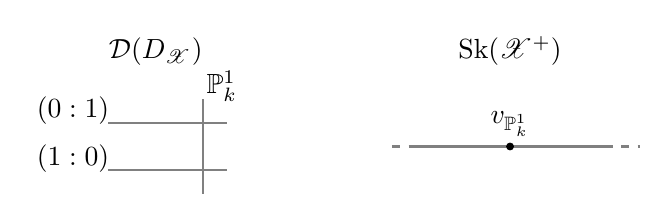
\begin{tikzpicture}[scale=0.3]
\draw[gray, thick] (-1,1) -- (-1,-3);
\draw[gray, thick] (-5,0) -- (0,0);
\draw[gray, thick] (-5,-2) -- (0,-2);
\node[above] at (-6.5,-0.5) {$(0:1)$};
\node[above] at (-6.5,-2.5) {$(1:0)$};
\node[above] at (-0.2,0.5) {$\mathbb{P}{^1_k}$};
\node[above] at (-3,2) {$\mathcal{D}(D_\cX)$};
\draw[gray, thick] (8,-1) -- (12,-1) -- (16,-1);
\draw [gray, thick, dashed] (7,-1) -- (8,-1);
\draw [gray, thick, dashed] (16,-1) -- (17.5,-1);
\filldraw[black] (12,-1) circle (4pt) node[above] {$v_{\mathbb{P}^1_k}$};
\node[above] at (12,2) {$\Sk(\cX^+)$};
\end{tikzpicture}
\end{center}
Since $\divisor_{\cX^+}(\omega)= 0$, the weight associated to $\omega$ is minimal at any point of the skeleton $\Sk(\cX^+)$. Thus $\Sk(X,\Delta_X,\omega)=\Sk(\cX^+)$.
\end{example}
\begin{example}
Let $X=\mathbb{P}^1_K$ and $\Delta_X=\frac{1}{2}(0:1) + \frac{1}{2}(1:0)+\frac{1}{2}(1:1)+\frac{1}{2}(-1:1)$. So $a_i=\frac{1}{2}$ for any $i$ and there exist $\Delta_X$-logarithmic $2$-pluricanonical forms. We set $$\omega = \frac{1}{x+1} \cdot \frac{1}{x-1} \cdot \frac{1}{x} (dx)^2= \frac{1}{y+1} \cdot \frac{1}{1-y}\cdot \frac{1}{y} (dy)^2.$$ We consider $\cX= \mathbb{P}_R^1$ and $D_\cX= (0:1) + (1:0)+ (1:1)+(-1:1)+ \mathbb{P}^1_k$, then $\cX^+=(\cX,D_\cX)$ is a log-regular model of $X^+=(X,\lceil \Delta_X \rceil)$ and $\Sk(\cX^+)$ is \begin{center}
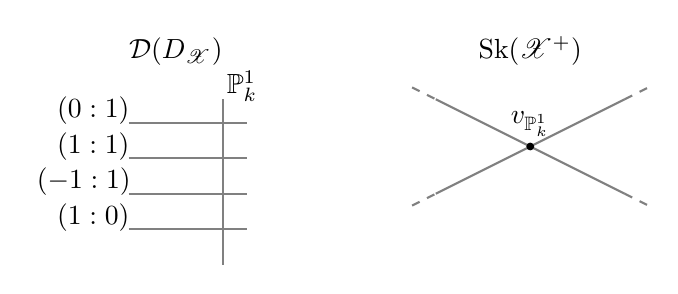
\begin{tikzpicture}[scale=0.3]
\draw[gray, thick] (-1,1) -- (-1,-6);
\draw[gray, thick] (-5,0) -- (0,0);
\draw[gray, thick] (-5,-1.5) -- (0,-1.5);
\draw[gray, thick] (-5,-3) -- (0,-3);
\draw[gray, thick] (-5,-4.5) -- (0,-4.5);
\node[above] at (-6.5,-0.5) {$(0:1)$};
\node[above] at (-6.5,-2) {$(1:1)$};
\node[above] at (-6.9,-3.5) {$(-1:1)$};
\node[above] at (-6.5,-5) {$(1:0)$};
\node[above] at (-0.2,0.5) {$\mathbb{P}{^1_k}$};
\node[above] at (-3,2) {$\mathcal{D}(D_\cX)$};
\draw[gray, thick] (8,1) -- (12,-1);
\draw[gray, thick] (16,1) -- (12,-1);
\draw[gray, thick] (8,-3) -- (12,-1);
\draw[gray, thick] (16,-3) -- (12,-1);
\draw [gray, thick, dashed] (7,1.5) -- (8,1);
\draw [gray, thick, dashed] (16,1) -- (17,1.5);
\draw [gray, thick, dashed] (7,-3.5) -- (8,-3);
\draw [gray, thick, dashed] (16,-3) -- (17,-3.5);
\filldraw[black] (12,-1) circle (4pt) node[above] {$v_{\mathbb{P}^1_k}$};
\node[above] at (12,2) {$\Sk(\cX^+)$};
\end{tikzpicture}
\end{center}
Since $\divisor_{\cX^+}(\omega)= (0:1) + (1:0)+ (1:1)+(-1:1)$, the weight associated to $\omega$ is minimal at the divisorial point $v_{\mathbb{P}_k^1}$ corresponding to $\mathbb{P}^1_k$ and is strictly increasing with slope $1$ along the unbounded edges, when we move away from the point $v_{\mathbb{P}^1_k}$. Therefore, $\Sk(X,\Delta_X,\omega)=\{v_{\mathbb{P}^1_k}\}$.
\end{example}

\subsection{Weight function for log-regular models.}
\spa{In case the divisor $\Delta_X$ is empty, the forms we considered in the previous paragraph to construct the weight functions are simply the sections of the $m$-pluricanonical line bundle $\omega_{X/K}^{\otimes m}$ on $X$, for some $m>0$. Given a $m$-pluricanonical form $\omega$ on $X$, we check that the weight function $\weight_{\omega}$ defined as in (\ref{equ:weight function formula}) coincides with the definition of the weight function associated to $\omega$ according to \cite{MustataNicaise}. This results in a generalized formula for the usual weight of $\omega$ at the birational points, in terms of their representations in skeleta associated to log-regular models of $X$.}

\begin{prop} \label{prop weight function log formula}
Let $\cX$ be a model of $X$ over $R$ such that $\cX^+$ is log-regular over $S^+$. If $x$ is a point of $\Sk(\cX^+)$, then the weight of $\omega$ at $x$ as in \cite{MustataNicaise} is given by $$\weight_{\omega}(x)=v_x(\divisor_{\cX^+}(\omega)) +m.$$
\end{prop}
\begin{proof}
In order to compute the weight of $\omega$ at $x$ according to the definition in \cite{MustataNicaise}, we can consider any snc model $\cY$ of $X$ such that $x$ is a point of $\Sk(\cY)$. Then, by \cite{NicaiseXu}, Section 3.2.2, the weight is given by $$v_x(\divisor_{\cY^+}(\omega))+m.$$
As we noticed in Remark \ref{rem resolution via subd}, we can obtain an snc model $\cY$ adapted to $x$ by means of a log blow-up $h: \cY^+ \rightarrow \cX^+$ of $\cX^+$ (Propositions \ref{resolution log scheme kato fan} and \ref{prop morphism induced by subdivision kato fan}). Moreover, the corresponding skeleton $\Sk(\cY^+)$ is given by a subdivision of $\Sk(\cX^+)$ (Proposition \ref{kato subdivision}) and coincides with $\Sk(\cY)$. Therefore it suffices to prove that $v_x(\divisor_{\cY^+}(\omega)) =   v_x(\divisor_{\cX^+}(\omega))$ for such a model $\cY^+$.

Log blow-ups are log-\'{e}tale morphisms (\cite{Saito2004}, Section 2.1) and for log-\'{e}tale morphisms the sheaf of log differentials is stable under pullback (\cite{Kato1994a}, Proposition 3.12), therefore $$h^* \omega_{\cX^+/ S^+}^{\text{log}} \simeq \omega_{\cY^+/S^+}^{\text{log}}.$$ Then $\divisor_{\cY^+}(\omega)=h^* \divisor_{\cX^+}(\omega)$ and in particular for points $x$ of the skeleton $\Sk(\cX^+) = \Sk(\cY)$, it holds that $$v_{x}(\divisor_{\cY^+}(\omega))= v_{x}(h^*\divisor_{\cX^+}(\omega))= v_x(\divisor_{\cX^+}(\omega)).$$
\end{proof}


\subsection{Weight function and Kontsevich-Soibelman skeleton for products.} \label{paragraph weight function product}
\spa{Let $\cX^+$ and $\cY^+$ be log-smooth models over $S^+$ of $X^+=(X,\lceil\Delta_X\rceil)$ and $Y^+=(Y,\lceil\Delta_Y\rceil)$ respectively. Then, the $fs$ fibred product $\cZ^+=\cX^+  \times^{\text{fs}}_{S^+} \cY^+$ is a log-regular model of $Z^+:=X^+ \times^{\text{fs}}_K Y^+$. Therefore, given $\omega_{X^+}$ and $\omega_{Y^+}$ $\Delta_X$-logarithmic and $\Delta_Y$-logarithmic $m$-pluricanonical forms on $(X,\Delta_X)$ and $(Y,\Delta_Y)$ respectively, the form $$\varpi=\pr_{X^+}^* \,\omega_{X^+} \otimes \pr_{Y^+}^* \,\omega_{Y^+}$$ is a $\Delta_Z$-logarithmic $m$-pluricanonical form on $(Z,\Delta_Z)$, where $\Delta_Z= X \times_K \Delta_Y + \Delta_X \times_K Y$. Viewing these forms as rational sections of logarithmic $m$-pluricanonical bundles, we see that $\divisor_{\cZ^+}(\varpi)=\divisor_{\cZ^+}( \pr_{X^+}^* \,\omega_{X^+} \otimes \pr_{Y^+}^* \,\omega_{Y^+})$ according to (\ref{equ log can bundles}).}

\spa{Let $z$ be a point of $F_{\cZ}$; as before, we denote by $x$ and $y$ the images of $z$ under the local isomorphism $F_{\cZ} \rightarrow F_{\cX} \times F_{\cY}$. Any morphism $\varepsilon \in \sigma_z$ defines a point $v_{z,\varepsilon}$ in $\Sk(\cZ^+)$. For the sake of convenience, we simply denote the valuations by the corresponding morphisms and we denote $\alpha= \pr_{\cX}(\varepsilon)$ and $\beta=\pr_{\cY}(\varepsilon)$. We aim to relate the valuation $v_{\varepsilon}\big(\divisor_{\cZ^+}(\varpi)\big)$ to the values $$v_{\alpha}\big(\divisor_{\cX^+}(\omega_{X^+}\big)) \text{ , } v_{\beta}\big(\divisor_{\cY^+}(\omega_{Y^+})\big).$$}

\spa{Let $f_x \in \caO_{\cX,x}$ be a local equation of $\divisor_{\cX^+}(\omega_{X^+})$ around $x$. In order to evaluate $v_{x,\alpha}$ on $f_x$, we consider an admissible expansion of $f_x$ as in (\ref{eq-adm}) $$f_x=\sum_{\gamma\in \caC_{\cX,x}}c_\gamma \gamma.$$ Furthermore, this expansion induces also an expansion of $\pr_{\cX}^*(f_x)$ by  $$\pr_{\cX}^*(f_x)=\sum_{\gamma\in \caC_{\cX,x} }\pr^*_{\cX}(c_\gamma) \gamma$$ as formal power series in $\widehat{\caO}_{\cZ,z}$, since the morphism of characteristic sheaves $\mathcal{C}_{\cX,x} \hookrightarrow \mathcal{C}_{\cZ,z}$ is injective. Following the same procedure for a local equation $f_y \in \caO_{\cY,y}$ of $\divisor_{\cY^+}(\omega_{Y^+})$ around $y$, we get an expansion of $f_y$ that extends to $\pr_{\cY}^*(f_y)$: 
$$f_y=\sum_{\delta\in \caC_{\cY,y}}d_\delta \delta.$$}

\spa{A local equation of $\varpi$ around $z$ is determined by $\pr_{\cX}^*(f_x)\,\,\pr_{\cY}^*(f_y)$. Thus $$v_{\varepsilon}(\divisor_{\cZ^+}(\varpi))
= v_{\varepsilon}\big(\pr_{\cX}^*(f_x) \,\,\pr_{\cY}^*(f_y)\big)$$ and by multiplicativity of the valuation $v_{\varepsilon}$ $$v_{\varepsilon}\big(\pr_{\cX}^*(f_x) \,\,\pr_{\cY}^*(f_y)\big) = v_{\varepsilon}\big(\pr_{\cX}^*(f_x)\big) + v_{\varepsilon}\big(\pr_{\cY}^*(f_y)\big).$$ Recalling Remark \ref{rem def-val}, the valuation can be computed as follows $$ v_{\varepsilon}\big(\pr_{\cX}^*(f_x)\big) = \min\{\varepsilon(\gamma)\,|\,c_\gamma \neq 0\};$$ as the elements $\gamma$ belong to $\caC_{\cX,x}$ and $\alpha$ is defined to be $\pr_{\cX}(\varepsilon)$ $$\min\{\varepsilon(\gamma)\,|\,c_\gamma \neq 0\} = \min\{\alpha(\gamma)\,|\,c_\gamma \neq 0\} =  v_{x,\alpha}(f_x).$$ Hence, we conclude that \begin{align} \label{equ valuations product}
\begin{split}
v_{\varepsilon}\big(\divisor_{\cZ^+}(\varpi)\big)
& = v_{\varepsilon}\big(\pr_{\cX}^*(f_x)\big) + v_{\varepsilon}\big(\pr_{\cY}^*(f_y)\big)\\
& = v_{\alpha}(f_x) + v_{\beta}(f_y) \\
& = v_{\alpha}\big(\divisor_{\cX^+}(\omega_{X^+})\big) + v_{\beta}\big(\divisor_{\cY^+}(\omega_{Y^+})\big).
\end{split}
\end{align}
}

\spa{This result turns out to be advantageous to compute the weight function $\weight_\varpi$ on divisorial points of $\Sk(\cZ^+)$: 
\begin{align} \label{equ weight function product}
\begin{split}
\weight_\varpi(\varepsilon)
& = v_{\varepsilon}\big(\divisor_{\cZ^+}(\varpi)\big) +m \\
& = v_{\alpha}\big(\divisor_{\cX^+}(\omega_{X^+})\big) + v_{\beta}\big(\divisor_{\cY^+}(\omega_{Y^+})\big) + m \\
& = \weight_{\omega_{X^+}}(\alpha) + \weight_{\omega_{Y^+}}(\beta) - m.
\end{split}
\end{align}
}


\spa{Under the notations of the previous paragraphs, our computations lead to the following result.
\begin{thm}  \label{thm semistability and KS skeleta}
Suppose that the residue field $k$ is algebraically closed and that $\cX^+$ is semistable. Then, the homeomorphism of skeleta $$\Sk(\cZ^+) \xrightarrow{\sim} \Sk(\cX^+) \times \Sk(\cY^+)$$ given in Proposition \ref{prop semistability and skeleta} restricts to a homeomorphism of Kontsevich-Soibelman skeleta $$\Sk(Z,\Delta_Z, \varpi) \xrightarrow{\sim} \Sk(X,\Delta_X, \omega_{X^+}) \times \Sk(Y,\Delta_Y, \omega_{Y^+}).$$ 
\end{thm}
\begin{proof}
This follows immediately from the equality (\ref{equ weight function product}) that shows that a point in $\Sk(Z,\Delta_Z)$ has minimal value $\weight_{\varpi}(Z,\Delta_Z)$ if and only if its projections have minimal value $\weight_{\omega_{X^+}}(X,\Delta_X)$ and $\weight_{\omega_{Y^+}}(Y,\Delta_Y)$.
\end{proof}
}

\section{The essential skeleton of a product}
We will need a few notions from birational geometry, see \cite{KollarMori}. Let $(X,\Delta_X)$ be a pair such that $X$ is normal, $\Delta_X$ is effective, and $K_X+\Delta_X$ is $\mathbb{Q}$-Cartier. Then we say that $(X,\Delta_X)$ is log canonical if for every log resolution $f \colon Z \to X$, in the formula

\[
K_Z+\Delta_Z = f^*(K_X+\Delta_X)+\sum a_D D,
\]
where $\Delta_Z$ is the strict transform of $\Delta_X$ plus the reduced exceptional divisor, all the $a_D$ are nonnegative. The sum ranges over all components of $\Delta_Z$. In fact the quantity $a_D$ depends only on the valuation corresponding to $D$, and this condition needs only be tested on a single log resolution.

We will be most interested in the case where $(X,\Delta_X)$ satisfies the stronger condtion of being divisorially log terminal, or dlt. A closed subset $Y \subset X$ is called a log canonical center if for some (respectively any) log resolution, $Y$ is the image of a divisor $D$ with $a_D=0$. The pair $(X,\Delta_X)$ is said to be dlt if for every log canonical center $Y$, there is a neighborhood of the generic point of $Y$ where $(X,\Delta_X)$ is snc.

\subsection{Essential skeleton of a pair.}
\spa{Let $(X,\Delta_X)$ be a pair such that $X^+=(X,\lceil \Delta_X \rceil)$ is a log-regular log scheme. Let $\omega$ be a non-zero regular $\Delta_X$-logarithmic $m$-pluricanonical form on $(X,\Delta_X)$. Let $\cX^+$ be a log-smooth model of $X^+$ over $S^+$. Then, the associated divisor $\divisor_{\cX^+}(\omega)$ is effective. There exist unique positive integers $d$ and $n$ such that the divisor $\divisor_{\cX^+}(\omega^{\otimes d} \pi^{-n})$ is effective and the multiplicity of some component of the special fibre is zero: we denote this divisor by $D_{\min}(\cX,\omega)$. It follows from the properties of the weight function (Paragraph \ref{paragraph weight function}) that for any $x \in \Sk(\cX^+)$ $$v_x(D_{\min}(\cX,\omega)) + dm = \weight_{\omega^{\otimes d}\pi^{-n}}(x)= d \cdot \weight_{\omega} + v_x(\pi^{-n}) = d \cdot \weight_{\omega}(x) -n.$$
}
\begin{lemma} \label{lemma characterization minimal points}
Let $v_{x,\alpha}$ be a divisorial point in $\Sk(\cX^+)$, then $v_{x,\alpha} \in \Sk(X,\Delta_X, \omega)$ if and only if $D_{\min}(\cX,\omega)$ does not contain $x$.
\end{lemma}
\begin{proof}
We denote $v_{x,\alpha}$ simply by $\alpha$. By the above series of equalities, the weight function $\weight_{\omega}$ reaches its minimum at $\alpha$ if and only if $v_\alpha(D_{\min}(\cX,\omega))$ is minimal, hence in particular equal to zero.

Let $h: \cY^+ \rightarrow \cX^+$ be a sequence of blow-up morphisms of strata of $D_\cX$ such that $\alpha$ corresponds to an irreducible component $E$ of $D_\cY$. As in the proof of Proposition \ref{prop weight function on log regular model} $$h^*(D_{\min}(\cX,\omega))=h^*(\divisor_{\cX^+} (\omega^{\otimes d} \pi^{-n}))= \divisor_{\cY^+} (\omega^{\otimes d} \pi^{-n}).$$ Therefore we have that $v_\alpha(D_{\min}(\cX,\omega)) >0$ if and only if $E \subseteq \divisor_{\cY^+} (\omega^{\otimes d} \pi^{-n})$, and this holds if and only if $x \in D_{\min}(\cX,\omega)$.
\end{proof}

\spa{We define the essential skeleton $\Sk(X,\Delta_X)$ of $(X,\Delta_X)$ as the union of all Kontsevich-Soibelman skeleta $\Sk(X, \Delta_X,\omega)$, where $\omega$ ranges over all regular $\Delta_X$-logarithmic pluricanonical forms. 

The reason to define the essential skeleton this way is that it behaves nicely under birational morphisms. Let $f \colon X'\to X$ be a log resolution. Then there is a $\mathbb{Q}$-divisor $\Gamma$ with snc support, and no coefficient exceeding $1$, such that $K_{X'}+\Gamma' = f^*(K_X+\Delta_X)$. Take $\Delta_{X'}$ to be the positive part of $\Gamma'$.}
\begin{prop} \label{prop birational invariance essential skeleton for pairs}
Under the identification of the birational points of $X$ with those of $X'$, $\Sk(X, \Delta_X)$ is identified with $\Sk(X', \Delta_{X'})$.
\end{prop}
\begin{proof}
It suffices to check the proposition for divisorial valuations. By Lemma \ref{lemma characterization minimal points} a divisorial valuation $v$ is in the skeleton $\Sk(X,\Delta_X)$ if and only if there exists a log-regular model $\cX^+$ for $(X,\lceil\Delta_X\rceil)$ such that $v$ is a log canonical center of $(\cX, \Delta_X + \cX_{k,\redu})$, and there is a regular $\Delta_X$-logarithmic pluricanonical form $\omega$ whose divisor $D_{\min}(\cX,\omega)$ does not contain the center of $v$. As the essential skeleton $\Sk(X,\Delta_X)$ is a union of cells closed inside the skeleton associated to any log-regular model, we choose log-regular models $\cX^+$ and $\cX'^+$ so that $f$ extends to a log resolution $f_R \colon \cX' \to \cX$. We denote by $D = \overline{\Delta_X} + \cX_{k,\redu}$ and $D'=\overline{\Delta_{X'}} + \cX'_{k,\redu}$. 

Suppose $v$ is a divisorial point in $\Sk(X, \Delta_X) \cap \Sk(\cX^+)$. Then let $\omega$ be a $\Delta_X$-logarithmic $m$-pluricanonical form on $(X,\Delta_X)$ whose associated divisor $\divisor_{\cX^+}(\omega)$ in $\cX^+$ does not contain the center of $v$. As $(\cX, D)$ is a dlt pair, we have that $$K_{\cX'}+D'= f_R^*(K_{\cX}+D)+M$$ where $M$ is effective. Thus there is a $\Delta_{X'}$-logarithmic $m$-pluricanonical form $\omega'$ on $\cX'$, whose associated divisor $\divisor_{\cX'^+}(\omega')=f^*_R(\divisor_{\cX^+}(\omega))+mM$. As $v$ is a log canonical center of $(\cX,D)$, $M$ does not vanish along $v$, so neither does $\divisor_{\cX'^+}(\omega')$. Likewise $v$ is a log canonical center of $(\cX', D')$. It follows that $v \in \Sk(X',\Delta_{X'},\omega')$.

Conversely, for any $m$, pullback along with multiplication by the divisor of discrepancies $M$ induces an isomorphism of vector spaces $$H^0(\cX, mK_{\cX}+mD) \cong H^0(\cX', mK_{\cX'}+mD').$$ So if $v$ is a divisorial point in $\Sk(X', \Delta_{X'})$, it is a log canonical center of $(\cX, D')$ and there is a regular $\Delta_{X'}$-logarithmic $m$-pluricanonical form $\omega'$ not containing the center of $v$, for some $m>0$. As a result $v$ is also a log canonical center of $(\cX, D)$, so we need only to check the existence of a regular $\Delta_X$-logarithmic pluricanonical form on $\cX$ not vanishing at the center of $v$. We take the preimage of $\omega'$ in $H^0(\cX, mK_{\cX}+mD)$, and the associated divisor in $\cX$ must not contain the center of $v$ because its pullback does not.
\end{proof}

\spa{Suppose that $(X,\Delta_X)$ is a dlt pair over $K$, such that $K_X + \Delta_X$ is semiample. Suppose thar $\cX$ is a good dlt minimal model of $(X,\Delta_X)$ over $R$ and let $D=\overline{\Delta_X} + \cX_{k,\redu}$. We consider a log resolution $f:X' \rightarrow X$ that extends to a log resolution of $(\cX,D)$. We write $K_{X'} + \Gamma' = f^*(K_X + \Delta_X)$. Let $\Delta_{X'}$ be the positive part of $\Gamma'$. We may embed the open dual complex $\mathcal{D}_0^{=1}(\cX, D)$ into the birational points of $X$.
}
\begin{prop} \label{prop dual complex minimal good dlt = essential skeleton any resolution}
This embedding identifies $\mathcal{D}_0^{=1}(\cX, D)$ with $\Sk(X',\Delta_{X'})$.
\end{prop}
\begin{proof}
Choose a regular $R$-model $\cX'$ for $X'$ which is a log resolution of $(\cX, D)$ extending $f$ and let  $D'=\overline{\Delta_{X'}} + \cX'_{k,\redu}$, namely we have the log resolutions \begin{align*}
&(X', \Delta_{X'}) \rightarrow (X,\Delta_X) & \text{where }(X,\Delta_X) \text{ dlt and }\Delta_{X'} \text{ is the positive part of }\Gamma'\\
&(\cX', D') \rightarrow (\cX,D) & \text{where }D=\overline{\Delta_X} + \cX_{k,\redu} \text{ and } D'=\overline{\Delta_{X'}} + \cX'_{k,\redu}.
\end{align*} As in the previous proof, it suffices to check the proposition for divisorial valuations. Let $v$ be a divisorial valuation, and suppose $v \in \mathcal{D}_0^{=1}(\cX,D)$. Then $v$ is a log canonical center for $(\cX,D)$, so $v$ is also a log canonical center of $(\cX', D')$. For a sufficiently divisible index, we may find a $\Delta_X$-logarithmic pluricanonical form on $(X,\Delta_X)$ whose associated divisor in $\cX$ has vanishing locus $C$ such that $C$ is a divisor not containing the center of $v$. After pullback, we get a $\Delta_{X'}$-logarithmic pluricanonical form $\omega'$ whose associated divisor in $\cX'$ is supported on the strict transform of $C$ and the exceptional divisors of positive log discrepancy. But none of these contain $v$. Thus, $v \in \Sk(X',\Delta_{X'},\omega')$.

Conversely, if $v$ is a divisorial point in $\Sk(X', \Delta_{X'})$, then $v$ is a log canonical center of $(\cX', D')$, so $v$ is a log canonical center of $(\cX, D)$, hence an element of the open dual complex $\mathcal{D}_0^{=1}(\cX, D)$.
\end{proof}

\spa{We define the essential skeleton $\Sk(X,\Delta_X)$ of a dlt pair $(X, \Delta_X)$ as the essential skeleton of any log-resolution of $(X,\Delta_X)$: Proposition \ref{prop birational invariance essential skeleton for pairs} guarantees that this is well-defined. Thus, Proposition \ref{prop dual complex minimal good dlt = essential skeleton any resolution} compares the essential skeleton to the skeleton of a good minimal dlt model of $(X,\Delta_X)$. the result can be restated as follows: if $(X,\Delta_X)$ is a dlt pair with $K_X+\Delta_X$ semiample and $(\cX,D)$ is a good dlt minimal model of $(X,\Delta_X)$ over $R$, then $\mathcal{D}_0^{=1}(\cX, D) = \Sk(X,\Delta_X)$. This generalizes \cite{NicaiseXu}, Theorem 3.3.3 to dlt pairs.
}


\subsection{Essential skeleta and products of log-regular models.}

\spa{We say that a pair $(X,\Delta_X)$ has non-negative Kodaira-Iitaka dimension if some multiple of the line bundle $K_X + \Delta_X$ has a regular section.}
\begin{theorem} \label{thm essential skeleton of product via log-reg}
Assume that the residue field $k$ is algebraically closed. Let $(X,\Delta_X)$ and $(Y,\Delta_Y)$ be pairs such that $X^+=(X,\lceil \Delta_X \rceil)$ and $Y^+=(Y, \lceil \Delta_Y\rceil)$ are log-regular log scheme over $K$. Suppose that both pairs have non-negative Kodaira-Iitaka dimension and both admit log-regular models $\cX^+$ and $\cY^+$ over $S^+$, such that $\cX^+$ is semistable. Then, the homeomorphism of skeleta $$\Sk(\cZ^+) \xrightarrow{\sim} \Sk(\cX^+) \times \Sk(\cY^+)$$of Proposition \ref{prop semistability and skeleta} induces a homeomorphism of essential skeleta $$\Sk(Z,\Delta_Z) \xrightarrow{\sim} \Sk(X,\Delta_X) \times \Sk(Y,\Delta_Y)$$ where $\cZ^+$, $Z^+$ and $\Delta_Z$ are the respective products. 
\end{theorem}
\begin{proof}
It follows immediately from Theorem \ref{thm semistability and KS skeleta} that we have the inclusion $ \Sk(X,\Delta_X) \times \Sk(Y,\Delta_Y) \subseteq \Sk(Z,\Delta_Z)$. Thus, we reduce to prove the following statement. Let $v_{z,\varepsilon}$ be a divisorial point in $\Sk(\cZ^+)$ and $(v_{x,\alpha},v_{y,\beta})$ be the corresponding pair in $\Sk(\cX^+) \times \Sk(\cY^+)$ under the isomorphism of Proposition \ref{prop semistability and skeleta}; if $v_{z,\varepsilon}$ lies in the essential skeleton $\Sk(Z,\Delta_Z)$, then $v_{x,\alpha}$ lies in $\Sk(X,\Delta_X)$.

Assume that $v_{z,\varepsilon}$ lies in the essential skeleton $\Sk(Z,\Delta_Z)$. Then there exists a non-zero regular $\Delta_Z$-logarithmic $m$-pluricanonical form $\omega$ on $Z^+$, such that $v_{z,\varepsilon} \in \Sk(Z,\Delta_Z, \omega)$. By Lemma \ref{lemma characterization minimal points}, $D_{\min}(\cZ,\omega)$ does not contain $z$.

Let $E$ be an irreducible component of $\cY_k$ containing $y$ and denote by $\xi_E$ the generic point of $E$. Then the point in the Kato fan of $\cZ^+$ corresponding to $(x,\xi_E)$ is not contained in $D_{\min}(\cZ,\omega)$, as otherwise $z$ would be contained in it.

As $k$ is algebraically closed, we can choose a $k$-rational point $p$ in $E$ such that $p$ is contained in no other components of $D_\cY$ and $D_{\min}(\cZ,\omega)$ does not contained the locus $\overline{\{x\}} \times_R \{p\}$. By Hensel's Lemma, $p$ can be lifted to an $R$-rational point of $\cY$. The pull-back of $\cZ^+$ along this $R$-rational point is an embedding $i: \cX^+ \rightarrow \cZ^+$, so we have the diagram
\[
\xymatrix{ \cX^+ \ar[r]^i\ar[d] & \cZ^+ \ar[r]^{\pr_\cX}\ar[d]^{\pr_\cY} & \cX^+ \ar[d] \\
S \ar[r] & \cY^+\ar[r] & S.
}
\] Since $S$ has trivial normal bundle in $\cY$, we  have that $$\omega_{X^+/K}^{\log} = i^*\big(\omega_{Z^+/K}^{\log}\big),$$ so $i^*(\omega)$ is a non-zero regular logarithmic $m$-pluricanonical form on $X^+$ and in particular is a regular $\Delta_X$-logarithmic $m$-pluricanonical form. Moreover, $D_{\min}(\cX,i^*(\omega)) = i^*(D_{\min}(\cZ,\omega))$. Finally, $x$ is not contained in $D_{\min}(\cX, i^*(\omega))$, as otherwise $i(x)= \{x\} \times_R \{p\}$ would be contained in $D_{\min}(\cZ,\omega)$. By Lemma \ref{lemma characterization minimal points}, $x$ is a point of $\Sk(X,\Delta_X, i^*(\omega))$ and this concludes the proof.
\end{proof}
\begin{rem}
Consider the case where the line bundles $K_X + \Delta_X$ and $K_Y + \Delta_Y$ are semi-ample, i.e. some multiple of them is base point free. It follows from the arguments of \cite{NicaiseXu}, Theorem 3.3.3 that the essential skeleton of $(Z,\Delta_Z)$ is a finite union of Kontsevich-Soibelman skeleta where the union runs through a generating set of global sections of a sufficiently large multiple of $K_Z+\Delta_Z$. We can construct such a set from generating sets of global sections of multiples of $K_X + \Delta_X$ and $K_Y+ \Delta_Y$ respectively, via tensor product. Then, in this case, the result of Theorem \ref{thm essential skeleton of product via log-reg} follows directly from Theorem \ref{thm semistability and KS skeleta}.
\end{rem}


\subsection{Essential skeleta and products of dlt models.}

\begin{lemma}\label{smalltoric}
Let $M$ be the monoid generated by $r_1 \ldots r_{n_1}$, $s_1 \ldots s_{n_2}$ with the single relation $\sum_{i=1}^{n_1} r_i = \sum_{j=1}^{n_2} s_j$. Then any small $\mathbb{Q}$-factorialization of the affine toric variety $W=\Spec(k[M])$ associated to $M$ is a log resolution.
\end{lemma}

\begin{proof}
We calculate the fan of $W$. Let $N$ be the dual lattice of $M$. The fan associated to $W$ is the cone of elements of $N\otimes \mathbb{R}$ which are non-negative on $M$. We consider these as linear functions $l$ on the vector space spanned by the $r_i$ and $s_i$, subject to the restriction that $l(\sum_{i=1}^{n_1} r_i)=l( \sum_{j=1}^{n_2} s_j)$. Let $x_{ij}$ be the function which is $1$ on $r_i$ and $s_j$ and $0$ on all others. Then the fan of $W$ is given by the single cone $C_W$ spanned by the $x_{ij}$.

Any $\mathbb{Q}$-factorialization $\widetilde{W}$ corresponds to a simplicial subdivision of the cone $C_W$ (see \cite{Fulton1993}, p.65). We now check that every choice of $\widetilde{W}$ is non-singular.

A maximal cone of $\widetilde{W}$ is spanned by $n=n_1+n_2-1$ independent rays of $C_W$. Each ray of $C_W$ corresponds to a choice of $x_{ij}$, and we can index these by edges of the complete bipartite graph $B$ on the $r_i$ and $s_j$. These $x_{ij}$ are independent if and only if the corresponding edges form a spanning tree. Let $w_1 \ldots w_{n}$ span a maximal cone of $\widetilde{W}$. On this affine chart, $\widetilde{W}$ is smooth if and only if the $w_i$ generate $N$ as a lattice. We have shown already that the $x_{ij}$ generate $N$. But every $x_{ij}$ is either one of the $w_i$, or it completes a cycle in $B$, so that it is a $\mathbb{Z}$-linear combination of the $w_i$.
\end{proof}

\begin{prop}
Let $(\cX,\Delta_{\cX})$ and $(\cY,\Delta_{\cY})$ be semistable good projective dlt minimal pairs over the germ of a pointed curve $C$. The product $(\cZ,\Delta_{\cZ})$ is a log canonical pair, $K_\cZ+\Delta_{\cZ}$ is semiample, and the log canonical centers of $(\cZ,\Delta_{\cZ})$ are strata of the coefficient $1$ part of $\Delta_{\cZ}$.
\end{prop}

\begin{proof}
The product $\cZ$ is normal as $\cX$ and $\cY$ are semistable. The divisor $K_\cZ+\Delta_{\cZ}$ is semiample by pullback of semiample divisors.

Let $\widetilde{\cX}$ and $\widetilde{\cY}$ be log resolutions of $\cX$ and $\cY$. Then, we have 
\begin{align*}
K_{\widetilde{\cX}}+ \Delta_{\widetilde{\cX}}&= f_\cX^*(K_\cX + \Delta_{\cX}) + \sum a_i E_{\cX,i} \\
K_{\widetilde{\cY}}+ \Delta_{\widetilde{\cY}}&= f_\cY^*(K_\cY + \Delta_{\cY}) + \sum b_j E_{\cY,j}
\end{align*} where the coefficients $a_i$ and $b_j$ are non-negative. Let $\widetilde{\cZ}$ be a toroidal log resolution of the fs product $\widetilde{\cX} \times^{\text{fs}} \widetilde{\cY}$. In particular, $\widetilde{\cZ}$ is a log resolution of $\cZ$ and we can write $$K_{\widetilde{\cZ}}+ \Delta_{\widetilde{\cZ}}= f_\cZ^*(K_\cZ + \Delta_{\cZ}) + \sum c_h E_{\cZ,h}$$ where $\Delta_{\widetilde{\cZ}}$ is effective. Over the generic fibre, $(\cZ,\Delta_{\cZ})$ is dlt, so we need only compute discrepancies over the special fibre, namely study the positivity of the coefficients $c_h$. 

Let $\Gamma$ be a divisor of $\widetilde{\cZ}$ over the special fibre, denote by $v_\Gamma$ the corresponding divisorial valuation in $\Sk(\widetilde{\cZ}^+)$, by $\Gamma_\cX$, $\Gamma_\cY$ and $\Gamma_{\cZ}$ its images in $\cX$, $\cY$ and $\cZ$. The projections of $v_\Gamma$ in $\Sk(\widetilde{\cX}^+)$ and $\Sk(\widetilde{\cY}^+)$ are divisorial valuations. Up to subdivisions of the skeleta, we can assume without loss of generality that the projections correspond to divisors $\Gamma_{\widetilde{\cX}}$ and $\Gamma_{\widetilde{\cY}}$.

Choose a $\Delta_{\cX}$-logarithmic and a $\Delta_{\cY}$-logarithmic pluricanonical forms $\omega_{\cX}$ on $\cX$ and  $\omega_{\cY}$ on $\cY$ respectively, such that the divisors $\divisor_{\cX^+}(\omega_\cX)$ and $\divisor_{\cY^+}(\omega_{\cY})$ do not contain $\Gamma_\cX$ and $\Gamma_\cY$ respectively, where $\cX^+=(\cX,\lceil \Delta_{\cX}\rceil)$ and  $\cY^+=(\cY,\lceil \Delta_{\cY}\rceil)$. Then, the divisor $\divisor_{\cZ^+}(\omega_{\cZ})$, associated to the wedge product $\omega_{\cZ}$ of the pullbacks $\omega_{\cX}$ and $\omega_{\cY}$ to $\cZ$, does not contain $\Gamma_{\cZ}$.  Denote by $\omega_{\widetilde{\cX}}$, $\omega_{\widetilde{\cY}}$ and $\omega_{\widetilde{\cZ}}$ the pullback of the respective forms to $\widetilde{\cX}$, $\widetilde{\cY}$ and $\widetilde{\cZ}$. Then, we have 
\begin{align*}
\divisor_{\widetilde{\cX}^+} (\omega_{\widetilde{\cX}})&  = f_\cX^*(\divisor_{\cX^+}(\omega_\cX)) + \sum a_i E_{\cX,i} \\
\divisor_{\widetilde{\cY}^+} (\omega_{\widetilde{\cY}})&  = f_\cY^*(\divisor_{\cY^+}(\omega_\cY)) +  \sum b_j E_{\cY,j}\\
\divisor_{\widetilde{\cZ}^+} (\omega_{\widetilde{\cZ}})&  = f_\cZ^*(\divisor_{\cZ^+}(\omega_\cZ)) +  \sum c_h E_{\cZ,h}.
\end{align*} As $\divisor_{\cX^+}(\omega_\cX)$, $\divisor_{\cY^+}(\omega_{\cY})$ and $\divisor_{\cZ^+}(\omega_{\cZ})$ do not contain $\Gamma_\cX$, $\Gamma_\cY$ and $\Gamma_{\cZ}$ respectively, we have
\begin{align*}
v_{\Gamma_{\widetilde{\cX}}}(\divisor_{\widetilde{\cX}^+} (\omega_{\widetilde{\cX}}))&  = \sum a_i v_{\Gamma_{\widetilde{\cX}}}(E_{\cX,i}) \geqslant 0 \\
v_{\Gamma_{\widetilde{\cY}}}(\divisor_{\widetilde{\cY}^+} (\omega_{\widetilde{\cY}}))&  = \sum b_j v_{\Gamma_{\widetilde{\cY}}}(E_{\cY,j}) \geqslant 0\\
v_{\Gamma}(\divisor_{\widetilde{\cZ}^+} (\omega_{\widetilde{\cZ}}))&  = \sum c_h v_{\Gamma}( E_{\cZ,h}).
\end{align*}
From the formula \ref{equ valuations product},  $v_{\Gamma}(\divisor_{\widetilde{\cZ}^+} (\omega_{\widetilde{\cZ}}))= v_{\Gamma_{\widetilde{\cY}}}(\divisor_{\widetilde{\cY}^+} (\omega_{\widetilde{\cY}}))+ v_{\Gamma_{\widetilde{\cX}}}(\divisor_{\widetilde{\cX}^+} (\omega_{\widetilde{\cX}}))$, hence we obtain that the log discrepancy of $\Gamma$ with respect to the pair $(\cZ,\Delta_{\cZ})$ is non-negative. Moreover, it is zero if and only if the log discrepancies of $\Gamma_{\widetilde{\cX}}$ and $\Gamma_{\widetilde{\cY}}$ are both zero, namely if and only if $\Gamma_\cX$ and $\Gamma_{\cY}$ are log canonical centres of $(\cX,\Delta_{\cX})$ and $(\cY,\Delta_{\cY})$ respectively. Since for dlt pairs the log canonical centres are the strata of the coefficient $1$ part of the boundary, it follows that any log canonical centre of $(\cZ,\Delta_{\cZ})$ is a product of such strata, hence a stratum of the coefficient part $1$ of $(\cZ,\Delta_{\cZ})$.
\end{proof}
%
%\begin{theorem}
%$(Z, \Delta_Z)$ has a semistable good projective dlt minimal model $(Z', \Delta'_Z)$ and $\D^{=1}(\Delta'_Z) \cong \D^{=1}(\Delta_X) \times \D^{=1}(\Delta_Y)$.
%
%\end{theorem}
%
%\begin{proof}
%
%Let $\pi \colon W \to Z$ be a log resolution given by iterated blowups at centers of codimension $2$. Then there exists an effective divisor $D$ supported on all of the exceptional divisors such that $-D$ is $\pi$-ample. Let $B_X$ and $B_Y$ be effective Cartier divisors on $X$ and $Y$ whose respective supports are the boundary divisors of coefficient $1$. We may combine these to produce $B_Z$, an effective Cartier divisor on $Z$ whose support is the coefficient $1$ part of $\Delta_Z$.
%
%Choose $\epsilon$ small and rational. Then $\Gamma=\Delta_Z-B_Z$ is effective, and $(Z,\Gamma)$ is klt.
%
%There exists a divisor $\Gamma'$ on $W$ such that the difference between $\Gamma'$ and the pullback of $\Gamma$ is exceptional and 
%\[
%K_W+\Gamma' = \pi^*(K_Z+\Gamma).
%\]
%
%Take $\Gamma_W$ to be the positive part of $\Gamma_W$. Since $(Z,\Gamma)$ was klt, so is $(W,\Gamma_W)$. For sufficiently small $\delta$, $(W, \Gamma_W+\delta D)$ is still klt. Let $a_i$ be arbitrary small rational coefficients, one for each divisor of $\Delta_Z$ with coefficient $1$.
%
%We will recover our dlt model by running an MMP with scaling on the pair $(W, \Gamma_W+\delta D - \sum a_i \Delta_i)$, scaling with respect to an ample divisor $A$ equivalent to $-D$. By **BCHM** this MMP terminates in a log terminal model $\phi \colon W \dashrightarrow Z'$. Moreover, as long as the $a_i$ are small relative to $\delta$, when the MMP terminates it must be the case that every exceptional divisor is contracted.  As running MMP induces birational contractions, the morphism $\psi \colon Z' \to Z$ is small. Hence $(Z', \psi^*\Delta_Z)$ is log canonical, and every log canonical center dominates a stratum of the coefficient $1$ part of $(Z,\Delta_Z)$.
%
%By construction of $Z'$, the divisor $-\sum a_i \Delta_i + \mu \phi_* A$ is $\psi$-ample, where $\mu$ is arbitrarily small. But for $\mu$ small enough, we can absorb $\mu \phi_* A$ into the term $\delta D$. Thus in fact $-\sum a_i \Delta_i$ is $\psi$-ample.
%
%As a result we can represent $Z' = \Proj_Z \bigoplus_{m \geq 0} \mathcal{O}(-m(\sum a_i \Delta_i))$. At this point we may take an arbitrarily large Veronese subring and assume the $a_i$ are all integers. We show that $(Z', \psi^*\Delta_Z)$ is dlt and compute its dual complex by looking at a formal toric model.
%
%It suffices to check near $z$, the generic point of a log canonical center, thus a stratum, of $(Z,\Delta_Z)$. Let $x$ and $y$ be the generic points of the corresponding strata of $(X,\Delta_X)$ and $(Y, \Delta_Y)$. Let $E_x$ and $E_y$ be the monoids of effective Cartier divisors supported on the strata near $x$ and $y$ respectively. Then the corresponding monoid for $z$ is $\langle E_x \oplus E_y \rangle /(t_x=t_y)$, where $t_x$ and $t_y$ are the respective sums of strata in the special fibers.
%
%This monoid has the form $E \oplus \mathbb{N}^l$, where $l$ is the number of horizontal divisors containing $z$, and $E$ is a monoid of the type considered in Lemma \ref{smalltoric}. The toric variety $T_{E,k}=\Spec k[E \oplus \mathbb{N}^l$ is a formal local model for $Z$ near $z$. so it suffices to consider $T=\Proj_{T_{E,k}} \bigoplus_{m \geq 0} \mathcal{O}(-m(\sum a_i \Delta_i))$, where the $\Delta_i$ range over the corresponding torus invariant Weil divisors.
%
%The divisors corresponding to the $l$ generators of $\mathbb{N}^l$ are Cartier, so their contribution to $T$ is trivial. Hence we reduce to the case $l=0$. For sufficiently general choices for the $a_i$, the toric variety $T$ is simplicial, its fan being induced by the simplicial subdivision of the fan of $T_{E,k}$ such that the $a_i$ induce a strictly convex piecewise linear function. By Lemma \ref{smalltoric}, for any such model, $T$ is a smooth toric variety, hence its invariant divisors are snc. Thus $(Z', \psi^*\Delta_Z)$ is dlt.
%
%Moreover, for any pair of monomial valuations $(v_x, v_y)$ centered at $x$ and $y$, there is a unique cone of the fan of $T_{E,k}$ containing the corresponding point. This corresponds to a unique stratum of $(Z', \psi^*\Delta_Z)$ and a unique monomial valuation on that stratum. Thus the valuation restriction map on dual complexes is one-to-one. We conclude it is an isomorphism.
%\end{proof}

\section{Applications}
\subsection{Weight functions and skeleta for finite quotients}

\spa{Let $X$ be a connected, smooth  and proper $K$-variety and let $G$ be a finite group acting on $X$. Let $X^{\an}$ be the analytification of $X$. We recall that any point of $X^{\an}$ is a pair $(x,|\cdot|_x)$ with $x \in X$ and $|\cdot|_x$ an absolute value on the residue field $\kappa(x)$ that extends the absolute value on $K$. For any point $x$ of $X$, an element $g$ of the group $G$ induces an isomorphism between the residue fields $\kappa(x)$ and $\kappa(g \ldotp x)$, that we still denote by $g$. Then, the action of $G$ extends to $X^\an$ in the following way $$g \ldotp (x,|\cdot|_x) = ( g \ldotp x,  |\cdot|_x \circ g^{-1}).$$ In particular the action preserves the sets of divisorial and birational points of $X$.

Let $f: X \rightarrow Y=X/G$ be the quotient map of $K$-schemes, let $f^\an: X^\an \rightarrow Y^\an$ be the map of Berkovich spaces induced by functoriality and let $\tilde{f}: X^\an \rightarrow X^\an/G$ be the quotient map of topological spaces.
\begin{prop} (\cite{Berkovich}, Corollary 5) \label{prop Berk identification of quotient}
Under the above notations, there is a canonical homeomorphism between $X^\an/G $ and $Y^\an$ such that $\tilde{f}$ and $f^\an$ are identified.
\end{prop}
}

\spa{Let $y$ be a divisorial point of $Y^\an$ and consider a regular snc $R$-model $\cY$ of $Y$ adapted to $y$, i.e. such that $y$ is the divisorial point associated to $(\cY, E)$ for some irreducible component $E$ of $\cY_k$. We denote by $\cX$ the normalization of $\cY$ inside $K(X) $, where $K(\cY)=K(Y)=K(X)^{G} \hookrightarrow K(X)$.

We check that $\cX$ is an $R$-model of $X$; it is enough to show that the base change $\cX_K$ is isomorphic to $X$. We consider the following commutative diagram
\begin{center}$
\begin{gathered}
\xymatrixrowsep{1pc}
\xymatrixcolsep{1pc}\xymatrix{ 
\cX_K \ar[drr] \ar[dddr] & & \\
& X \ar@{.>}[r] \ar@{.>}[ul]\ar[d]^{f} & \cX \ar[d] \\
& Y \ar[r] \ar[d] & \cY  \ar[d]\\
& \Spec K \ar[r] & S \\
}
\end{gathered}$
\end{center} As the $X$ is a normal variety endowed with a morphism $X \rightarrow \cY$, by universal property of normalization, it factors uniquely through $\cX$ and the diagram is still commutative. Then by universal property of fibred product, there exists a morphism $X \rightarrow \cX_K$. Therefore, it suffices to prove that $$[K(X):K(\cX_K)]=1.$$ Indeed, if this is the case, then $X \rightarrow \cX_K$ is a finite birational morphism between normal varietes, hence an isomorphism.

The degree of the extension $[K(X):K(\cX_K)]$ may be computed on an affine open, so we assume that $\cY$ is an affine scheme with associated ring $K[\cY]$. Then we consider the diagram of inclusions
\begin{center} 
$ \xymatrixcolsep{-1pc} \xymatrixrowsep{1pc}\xymatrix{ 
& K(\cX)=K(\cX_K) \ar[dr] & \\
\widehat{K[\cY]}=K[\cX] \ar[rr] \ar[ru] & & K(X)\\
K[\cY] \ar[u] \ar[rr]& & K(\cY)=K(Y)=K(X)^{G} \ar[u]^{\text{finite} \deg} \\
}$
\end{center} As $K(X)$ is finite field extension of $K(\cY)$ and $K[\cX]$ the integral closure of $K[\cY]$ in $K(X)$, then $K(X)$ is the fraction field of $K[\cX]$. Thus, $K(\cX) = \text{Frac}(K[\cX])=K(X)$ and in particular we conclude that $[K(X):K(\cX_K)]=1.$
}
\begin{rem} \label{rem divisorial repre quotient}
This procedure of normalization illustrates a way to start with a regular snc $R$-model $\cY$ of $Y$ adapted to a point $y \in \text{Div}(Y)$ and construct an $R$-model $\cX$ of $X$ that, by normality, is regular at generic points of the special fibre $\cX_k$. 
\end{rem}

\begin{lemma} \label{lemma G invariant forms and weight function}
Let $\omega$ be a $m$-pluricanonical form on $X$. If $\omega$ is $G$-invariant, then the weight function associated to $\omega$ on the set of birational points is stable under the action of $G$. 
\end{lemma}
\begin{proof}
Let $x$ be a birational point of $X$ and $g$ an element of $G$. There exist snc models $\cX$ and $\cX'$ over $R$ such that $x \in \Sk(\cX)$ and $g \ldotp x \in \Sk(\cX')$. By replacing them by an snc model $\cY$ that dominates both $\cX$ and $\cX'$, we can assume that both points lies in $\Sk(\cY)$. The weights of $\omega$ at $x$ and $g \ldotp x$ can be computed using the formula \ref{equ:weight function formula}, so \begin{align*} \weight_{\omega}(g \ldotp x)& = v_{g \ldotp x}(\divisor_{\cY^+}(\omega)) + m  = v_{x}((g^{-1})^*\divisor_{\cY^+}(\omega)) + m  \\ & = v_{x}(\divisor_{\cY^+}(\omega)) + m = \weight_{\omega}(x) \end{align*} as $\omega$ is a $G$-invariant form. Thus we see that birational points in the same $G$-orbit have the same weight with respect to $\omega$. 
\end{proof}

\begin{cor} \label{cor:G inv forms and KS}
Let $\omega$ be a $G$-invariant pluricanonical form on $X$. Then the Kontsevich-Soibelman skeleton $\Sk(X,\omega)$ is stable under the action of $G$.
\end{cor}
\begin{proof}
This follows immediately from Lemma \ref{lemma G invariant forms and weight function}.
\end{proof}

\begin{prop} \label{prop:G inv form and corresponding weights}
Let $\omega$ be a $G$-invariant $m$-pluricanonical form on $X$. Let $y$ be a divisorial point of $Y^\an$. Then, for any divisorial point $x \in (f^\an)^{-1}(y)$, the weights of $\omega$ at $x$ and $y$ coincide.
\end{prop}
\begin{proof}
Let $\cY$ be a regular snc $R$-model such that $y$ has divisorial representation $(\cY,E)$. Let $\cX$ be the normalization of $\cY$ in $K(X)$: as we observed in Remark \ref{rem divisorial repre quotient}, it is an $R$-model of $X$, regular at generic points of the special fibre $\cX_k$. The preimage of $E$ coincides with the pull-back of the Cartier divisor $E$ on $\cX$, hence $f^{-1}(E)$ still defines a codimension one subset on $\cX$. We denote by $F_i$ the irreducible components of $f^{-1}(E)$ and we associate to $F_i$'s their corresponding divisorial valuations $x_i=(\cX,F_i)$. By Lemma \ref{lemma G invariant forms and weight function}, it is enough to prove the result for one of the $x_i$'s. We denote it by $x = (\cX,F)$ and we compare the weights of $\omega$ at $y$ and $x$, namely
$$\weight_{\omega}(x)=v_{x}(\divisor_{\cX^+}(\omega)) +m \quad \text{ and} \quad \weight_{\omega}(y)=v_{y}(\divisor_{\cY^+}(\omega)) +m. $$ We recall that for log-\'{e}tale morphisms the sheaves of logarithmic differentials are stable under pull-back (\cite{Kato1994a}, Proposition 3.12). Furthermore, it suffices to check that, locally around the generic point of $F_i,$ the morphism $\cX^+ \rightarrow \cY^+$ is a log-\'{e}tale morphism of divisorial log structures, to conclude that the weights coincide. To this purpose, we will apply Kato's criterion for log \'{e}taleness (\cite{Kato1989}, Theorem 3.5) to log schemes with respect to the \'{e}tale topology.

We denote by $\xi_{F}$ the generic point of $F$ and by $\xi_E$ the generic point of $E$. The divisorial log structures on $\cX^+$ and $\cY^+$ have charts $\N$ at $\xi_{F}$ and $\xi_E$. In the \'{e}tale topology, the normalization morphism $\cX^+ \rightarrow \cY^+$ admits a chart induced by $t:\N \rightarrow \N$ where $1 \mapsto m$ for some positive integer $m$:
\begin{center}
$\xymatrix{
\Spec \caO_{\cX, \xi_{F}} \ar[d] \ar[r] & \Spec \Z[\N] \ar[d] \\
\Spec \caO_{\cY, \xi_{E}}  \ar[r] & \Spec \Z[\N] 
}$
\end{center} Firstly, by the universal property of the fibre product, we have a morphism $$\Spec \caO_{\cX, \xi_{F}} \rightarrow \Spec \caO_{\cY, \xi_{E}} \times_{\Spec \Z[\N] } \Spec \Z[\N]$$ and it corresponds to $$ \caO_{\cY, \xi_{E}}  \otimes_{\Z[\N]} \Z[\N] \rightarrow\caO_{\cX, \xi_{F}}.$$ This is a morphism of finite type with finite fibres between regular rings and by \cite{Liu2002}, Lemma 4.3.20 and \cite{Nowak} it is flat and unramified, hence \'{e}tale. One of the two conditions in Kato's criterion for log \'{e}taleness is then fulfilled. Secondly, the chart $t:\N \mapsto \N$ induces a group homomorphism $t^{\text{gp}}: \Z \mapsto \Z$; in particular, it is injective and it has finite cokernel. Then $t$ satisfies the second condition of Kato's criterion for log \'{e}taleness. Therefore we conclude that $\weight_\omega(y)=\weight_\omega(x)$.
\end{proof}

\begin{prop} \label{prop:G inv and homeo KS of quotient}
Let $\omega$ be a $G$-invariant pluricanonical form on $X$. Then the canonical homeomorphism between $X^\an/G$ and $Y^\an$ of Proposition \ref{prop Berk identification of quotient} induces the homeomorphism $$\Sk(X,\omega)/G \simeq \Sk(X/G,\omega).$$
\end{prop}
\begin{proof}
This follows immediately from Corollary \ref{cor:G inv forms and KS} and Proposition \ref{prop:G inv form and corresponding weights}.
\end{proof}

\spa{Let $X$ be a smooth $K$-variety and let $\omega_X$ be a pluricanonical form on $X$. Let $\pr_j:X^n \rightarrow X$ be the $j$-th canonical projection. Then $$\omega= \bigwedge_{1\leqslant j \leqslant n} \pr_j^*\omega_X$$ is a pluricanonical form on $X^n$ and moreover it is invariant under the action of $\mathfrak{S}_n$.
\begin{prop}  \label{prop semistability and KS symm quotient}
Assume that the residue field $k$ is algebraically closed.  If $X$ has semistable reduction \textcolor{red}{write right assumption}, then the Kontsevich-Soibelman skeleton of the $n$-th symmetric product of $X$ associated to $\omega$ is isomorphic to the $n$-th symmetric product of the Kontsevich-Soibelman skeleton of $X$ associated to $\omega_X$.
\end{prop}
\begin{proof}
Iterating the result of Theorem \textcolor{red}{reference}, we have that the projection map defines an isomorphism of Kontsevich-Soibelman skeleta $$\Sk(X^n, \omega) \xrightarrow{\sim} \Sk(X,\omega_X) \times  \ldots \times \Sk(X,\omega_X).$$ Thus, applying Proposition \ref{prop:G inv and homeo KS of quotient} with the group $\mathfrak{S}_n$ acting on the product $X^n$, we obtain that $$\Sk(X^n/\mathfrak{S}_n, \omega) \simeq \Sk(X^n,\omega)/\mathfrak{S}_n \simeq  \Sk(X,\omega_X)^n/ \mathfrak{S}_n$$
Since the action on the Kontsevich-Soibelman skeleton $\Sk(X^n,\omega)$ is induced from the symmetric action on $X^n$, and the projections $\pr_j:X^n \rightarrow X$ functorially induce the projections $\overline{\pr_j}: \Sk(X,\omega_X)^n \rightarrow \Sk(X,\omega)$, the action of $\mathfrak{S}_n$ on $\Sk(X,\omega)^n$ is exactly by permutations of the components. Thus, $$ \Sk(X,\omega_X)^n/ \mathfrak{S}_n \simeq \text{Sym}^n(\Sk(X,\omega_X)).$$
\end{proof}
}

\subsection{The essential skeleton of Hilbert schemes of a $\text{K3}$ surface} \label{sect essential sk Hilb}

\spa{Let $S$ be an irreducible regular surface. We consider $\Hilb^n(S)$ the Hilbert scheme of $n$ points on $S$: by \cite{Fogarty} it is an irreducible regular variety of dimension $2n$. Moreover, the morphism $$\rho_{HC}: \Hilb^n(S) \rightarrow S^n/\mathfrak{S}_n$$ that sends a zero-dimensional scheme $Z \subseteq S$ to its associated zero-cycle $\text{supp}(Z)$ is a birational morphism, called the Hilbert-Chow morphism.}

\spa{Let $S$ be a $\text{K}3$ surface over $K$, namely $S$ is a complete non-singular variety of dimension two such that $\Omega_{S/K}^2 \simeq \caO_S \text{ and } H^1(S,\caO_S) = 0$. In particular $S$ is a variety with trivial canonical line bundle. 
%We consider $\Hilb^n(S)$ the Hilbert scheme of $n$ points on $S$: by \cite{Fogarty} it is birational to the $n$-th symmetric product of $S$. Explicitely, the birational morphism $\rho: \Hilb^n(S) \rightarrow S^n/\mathfrak{S}_n$ sends a zero-dimensional scheme $Z \subseteq S$ to its associated zero-cycle $\text{supp}(Z)$. We refer to the morphism $\rho$ as the Hilbert-Chow morphism. 
% a concrete way to construct it is by first taking the $n$-th symmetric product of $S$, and by then resolving its singularities:
%\begin{center}
%$ \xymatrix{
%& S^n \ar[d]^{f} \\
%\Hilb^n(S) \ar[r]^{\rho} & S^n/\mathfrak{S}_n\\
%}$
%\end{center} Indeed, the $n$-th symmetric product $S^n/\mathfrak{S}_n$ has quotient singularities along the images via $f$ of the loci $$\Delta_{ij}= \{(x_1,\ldots,x_n) \in S^n \,|\, x_i=x_j\},$$ which are precisely the fixed loci of the $\mathfrak{S}_n$-action on $S^n$. Then the morphism $\rho: \Hilb^n(S) \rightarrow S^n/\mathfrak{S}_n$ is a resolution of singularities and it can be seen explicitly as the map sending a zero-dimensional scheme $Z \subseteq S$ to its associated zero-cycle $\text{supp}(Z)$. We refer to the morphism $\rho$ as the Hilbert-Chow morphism. It follows that the Hilbert scheme of $n$ points on $S$ is birational to the $n$-th symmetric product of $S$ \cite{Fogarty}. 
%We can finally illustrate the essential skeleton of the $n$-th Hilbert scheme of a $\text{K}3$ surface with semistable reduction.
\begin{cor}  \label{cor essential skeleton hilb}
Assume that $S$ has  semistable reduction and the residue field $k$ is algebraically closed. Then the essential skeleton of the Hilbert scheme of $n$ points on $S$ is isomorphic to the $n$-th symmetric product of the essential skeleton of $S$ $$\Sk(\Hilb^n(S)) \xrightarrow{\sim} \text{Sym}^n(\Sk(S)).$$ 
\end{cor}
\begin{proof}
This follows immediately from Corollary \ref{prop semistability and KS symm quotient} and the birational invariance of the essential skeleton, \cite{MustataNicaise}, Proposition 4.6.3.
\end{proof}
\begin{prop} \label{prop top essential skeleton Hilb}
If the essential skeleton of $S$ is homeomorphic to a point, a closed interval or the $2$-dimensional sphere, then the essential skeleton of $\Hilb^n(S)$ is homeomorphic to a point, the standard $n$-simplex or $\CP^n$ respectively. 
\end{prop}
\begin{proof} Applying Corollary \ref{cor essential skeleton hilb}, we reduce to the computation of the symmetric product of a point, a closed interval or the sphere $S^2$. Then, the result follows from \cite{Hatcher}, Section 4K.
\end{proof}

}

\subsection{The essential skeleton of generalised Kummer varieties} \label{sect essential sk Kummer}
\spa{Let $A$ be an abelian surface over $K$, namely a complete non-singular, connected group variety of dimension two. Since $A$ is a group variety, the canonical line bundle is trivial and the group structure provides a multiplication morphism $m_{n+1}: A \times A \times \ldots \times A \rightarrow A$ that is invariant under the permutation action of $\mathfrak{S}_{n+1}$, hence it induces a morphism $$\Sigma_{n+1}: \Hilb^{n+1}(A) \xrightarrow{\rho_{HC}} \text{Sym}^{n+1}(A) \rightarrow A$$ by composition with the Hilbert-Chow morphism. Then $\text{K}_n(A) = \Sigma_{n+1}^{-1}(1)$ is called the $n$-th generalised Kummer variety and is a hyper-K\"{a}hler manifold of dimension $2n$ (\cite{Beauville1983}).
}
\spa{In \cite{HalvardHalleNicaise2017}, Proposition 4.3.2, Halle and Nicaise, using Temkin's generalization of the weight function (\cite{Temkina}), prove that the essential skeleton of an abelian variety $A$ over $K$ coincides with the construction of a skeleton of $A$ done by Berkovich in \cite{Berkovich1990}, Paragraph 6.5. It follows from this identification and \cite{Berkovich1990}, Theorem 6.5.1 that the essential skeleton of $A$ has a group structure, compatible with the group structure on $A^\an$ under the retraction $\rho_A$ of $A^\an$ onto the essential skeleton, so the following diagram commutes
\begin{center}
$\xymatrix{
(A^\an)^{n+1} \ar[d]_{(\rho_A)^{n+1}} \ar[r]^-{m_{n+1}^\an} & A^\an \ar[d]^{\rho_A} \\
\Sk(A)^n \ar[r]^-{\mu_{n+1}} & \Sk(A)
}$
\end{center} where $\mu$ denotes the multiplication of $\Sk(A)$.
}
\begin{prop} \label{prop essential skeleton Kummer}
Let $A$ be an abelian surface over $K$. Assume that $A$ has  semistable reduction and the residue field $k$ is algebraically closed. Then the essential skeleton of the $n$-th generalised Kummer variety is isomorphic to the symmetric quotient of the kernel of the morphism $\mu$, namely $$\Sk(\text{K}_n(A)) \simeq \Sk\big(m_{n+1}^{-1}(1)/\mathfrak{S}_{n+1}\big) \simeq \mu_{n+1}^{-1}(1)/\mathfrak{S}_{n+1}.$$ 
\end{prop}
\begin{proof}
The first homeomorphism follows from the birational invariance of the essential skeleton (\cite{MustataNicaise}, Proposition 4.6.3). We denote by $$L=m_{n+1}^{-1}(1) \quad \text{ and }\quad \Lambda=\mu_{n+1}^{-1}(1).$$ For any choice of an $\mathfrak{S}_{n+1}$-invariant generating canonical form on $A$, it follows from Proposition \ref{prop:G inv and homeo KS of quotient} that $\Sk(L/\mathfrak{S}_{n+1}) \simeq \Sk(L)/\mathfrak{S}_{n+1}$. We reduce to study the quotients $\Sk(L)/\mathfrak{S}_{n+1}$ and $\Lambda/\mathfrak{S}_{n+1}$.

Let $\mathfrak{S}_n'$ and $\mathfrak{S}_n''$ be the subgroups of $\mathfrak{S}_{n+1}$ of the permutations that fix $n$ and $n+1$ respectively. Then $\mathfrak{S}_{n+1}$ is generated by the two subgroups, so its action on $\Sk(L)$ and $\Lambda$ is completely determined by the actions of these subgroups. We consider the following isomorphisms 
\begin{align*}
f_n: &L \xrightarrow{\sim} A^n \quad (z_1,\ldots,z_{n+1}) \mapsto (z_1,\ldots,z_{n-1},z_{n+1}) \\
f_{n+1}: &L \xrightarrow{\sim} A^n \quad (z_1,\ldots,z_{n+1}) \mapsto (z_1,\ldots,z_{n-1},z_{n}).
\end{align*} Then $f_n$ is $\mathfrak{S}_n'$-equivariant, $f_{n+1}$ is $\mathfrak{S}_n''$-equivariant and the morphism $\psi$
\begin{center}
\xymatrixrowsep{0.1pc} $\xymatrix{
& L  \ar[ldd]_{f_{n+1}} \ar[ddr]^{f_n} &\\
& & \\
A^n \ar[rr]^{\psi}& & A^n \\
(z_1,\ldots,z_{n-1},z_{n}) \ar@{|->}[rr]& & (z_1,\ldots, \prod_{i=1}^{n} z_i^{-1}).
}$
\end{center} is equivariant with respect to the action of $\mathfrak{S}_n''$ on the source and of $\mathfrak{S}_n'$ on the target. Hence, we obtain a commutative diagram of equivariant isomorphisms. We denote by $\overline{f}_n$, $\overline{f}_{n+1}$ and $\overline{\psi}$ the isomorphisms induced on the essential skeleta. By Theorem \textcolor{red}{reference} we can identify $\Sk(A^n)$ with $\Sk(A)^n$. Thus, we have the commutative diagram
\begin{center}
\xymatrixrowsep{0.1pc} $\xymatrix{
& \Sk(L)  \ar[ldd]_{\overline{f}_{n+1}} \ar[ddr]^{\overline{f}_n} &\\
& & \\
\Sk(A)^n \ar[rr]^{\overline{\psi}}& & \Sk(A)^n \\
(v_1,\ldots,v_{n-1},v_{n}) \ar@{|->}[rr]& & (v_1,\ldots, \prod_{i=1}^{n} v_i^{-1}).
}$
\end{center} Then the action of $\mathfrak{S}_{n+1}$ on $\Sk(L)$ is induced by the isomorphisms $\overline{f}_n$ and $\overline{f}_{n+1}$ from the actions of $\mathfrak{S}_n''$ and $\mathfrak{S}_n'$ on $\Sk(A)^n$ and these actions are compatible as $\overline{\psi}$ is equivariant.

In a similar way, $\Lambda$ is isomorphic to $n$ copies of $\Sk(A)$ and comes equipped with an action of $\mathfrak{S}_{n+1}$. So, we have equivariant projections $g_n$ and $g_{n+1}$ with respect to $\mathfrak{S}_n'$ and $\mathfrak{S}_n''$. The equivariant morphism that completes and makes the diagram commutative is $\overline{\psi}$. Finally, we have the equivariant commutative diagram
\begin{center}
\xymatrixrowsep{1pc}
\xymatrixrowsep{1pc}
$\xymatrix{
& \Sk(L)  \ar[ld]_{\overline{f}_{n+1}} \ar[rd]^{\overline{f}_{n}}  &\\
\mathfrak{S}_n'' \circlearrowleft\Sk(A)^n  \ar[rr]^{\overline{\psi}}& & \Sk(A)^n\circlearrowright \mathfrak{S}_n' \\
& \Lambda\ar[lu]^{g_{n+1}}\ar[ru]_{g_n} &
}$
\end{center} and we conclude that the quotients $\Sk(Z)/\mathfrak{S}_{n+1}$ and $\Lambda/\mathfrak{S}_{n+1}$ are homeomorphic.
\end{proof}

\begin{prop} \label{prop top essential skeleton Kummer}
If the essential skeleton of $A$ is homeomorphic to a point, the circle $S^1$ or the torus $S^1 \times S^1$, then the essential skeleton of $\text{K}_n(A)$ is homeomorphic to a point, the standard $n$-simplex or $\CP^n$ respectively. 
\end{prop}
\begin{proof}
The case of the point is trivial. For the circle $S^1$, it follows directly from \cite{Morton}, Theorem. To prove the result for the torus $S^1 \times S^1$, we apply \cite{Looijenga}, Theorem 3.4: the action of the symmetric group corresponds to the root system of $A_n$, the highest root is the sum of the simple roots, each with coefficient $1$, and so the quotient is the complex projective space of dimension $n$.

\textcolor{red}{add comment to the proof}
\end{proof}

\subsection{Remarks}
\spa{The cases we consider in Proposition \ref{prop top essential skeleton Hilb} and Proposition \ref{prop top essential skeleton Kummer} are motivated by the work of Kulikov, Persson and Pinkham. In \cite{Kulikov} and \cite{PerssonPinkham1981}, they consider degenerations  over the unit complex disk, of surfaces such that some power of the canonical bundle is trivial. They prove that, after base change and birational transformations, any such degeneration can be arranged to be semistable with trivial canonical bundle, namely a \emph{Kulikov degeneration}. Then, they classify the possible special fibres of Kulikov degenerations according to the type of the degeneration.

We recall that the monodromy operator $T$ on $\text{H}^2(X_t, \Q)$ of the fibres $X_t$ of a Kulikov degeneration is unipotent, so we denote by $\nu$ the nilpotency index of $\log(T)$, namely the positive integer such that $\log(T)^\nu=0$ and $\log(T)^{(\nu-1)} \neq 0$. The type of the Kulikov degeneration is defined as the nilpotency index $\nu$ and called type I, II or III accordingly to it.

It follows from \cite{Kulikov}, Theorem II, that the dual complex of the special fibre of a Kulikov degeneration of a $\text{K}3$ surface is a point, a closed interval or the sphere $S^2$ according to the respective type. For a degeneration of abelian surfaces, the dual complex of the special fibre is homeomorphic to a point, the circle $S^1$ or the torus $S^1 \times S^1$ according to the three types (see an overview of these results in \cite{FriedmanMorrison}). In all cases, the dimension of the dual complex is equal $\nu-1$, hence determined by the type.
}

\spa{Hilbert schemes of $\text{K}3$ surfaces and generalised Kummer varieties represent two families of examples of hyper-K\"{a}hler varieties. For a semistable degeneration of hyper-K\"{a}hler manifolds over the unit disk, it is possible to define the type as the nilpotency index of the monodromy operator on the second cohomology group. It naturally extends the definition for Kulikov degenerations.
%In particular, the nilpotency index of the monodromy of a degeneration of a $\text{K}3$ surface coincides with the nilpotency index of the monodromy of the corresponding degeneration of the Hilbert scheme (\cite{Beauville1983}, Lemma 2), so the corresponding degenerations are of the same type.

In \cite{KollarLazaSaccaEtAl2017}, Koll\'{a}r, Laza, Sacc\`{a} and Voisin study the essential skeleton of a degeneration of hyper-K\"{a}hler manifolds in terms of the type. More precisely, in Theorem 0.10, given a minimal dlt degeneration of $2n$-dimensional hyper-K\"{a}hler manifolds, firstly they prove that the dual complex of the special fibre has dimension $(\nu-1)n$, where $\nu$ denotes the type of the degeneration. Secondly, they prove that, in the type III case, the dual complex is a simply connected closed pseudo-manifold with the rational homology of $\CP^n$.

From this prospective, Proposition \ref{prop top essential skeleton Hilb} and Proposition \ref{prop top essential skeleton Kummer} confirm and strengthen their result for the specific cases of Hilbert schemes and generalized Kummer varieties. In particular, we turn the rational cohomological description of the essential skeleton (Theorem 0.10(ii)) into a topological characterization.

For Hilbert schemes associated to some type II degenerations of $\text{K}3$ surfaces, a complementary proof of our result is due to Gulbrandsen, Halle, Hulek and Zhang, see \cite{GulbrandsenHalleHulek2016} and \cite{GulbrandsenHalleHulekEtAl}. Their approach is based on the method of \textit{expanded degenerations}, which first appeared in \cite{Li}, and on the construction of suitable GIT quotients, in order to obtain an explicit minimal dlt degeneration for the associated family of Hilbert schemes.
}
\spa{The structure of the essential skeleton of a degeneration of hyper-K\"{a}hler manifolds is relevant in the context of mirror symmetry and in view of the work of Kontsevich and Soibelman (\cite{KontsevichSoibelmana}, \cite{KontsevichSoibelman}). The SYZ fibration (\cite{StromingerYauZaslow}) is a conjectural geometric explanation for the phenomenon of mirror symmetry and, roughly speaking, asserts the existence of a special Lagrangian fibration, such that mirror pairs of manifolds with trivial canonical bundle should admit fibrewise dual special Lagrangian fibrations. Moreover, the expectation is that, for type III degenerations of $2n$-dimensional hyper-K\"{a}hler manifolds, the base of the SYZ fibration is $\CP^n$ (see for instance \cite{Hwang}).

The most relevant fact from our prospective is that Kontsevich and Soibelman predict that the base of the Lagrangian fibration of a type III degeneration is homeomorphic to the essential skeleton. So, the outcomes on the topology of the essential skeleton we obtain in Proposition \ref{prop top essential skeleton Hilb} and Proposition \ref{prop top essential skeleton Kummer} match the predictions of mirror symmetry about the occurrence of $\CP^n$ in the type III case. 
}
\printbibliography 
\end{document}